%% For double-blind review submission
\documentclass[sigplan,10pt,review,anonymous]{acmart}\settopmatter{printfolios=true}
%% For single-blind review submission
%\documentclass[sigplan,10pt,review]{acmart}\settopmatter{printfolios=true}
%% For final camera-ready submission
%\documentclass[sigplan,10pt]{acmart}\settopmatter{}

%% Note: Authors migrating a paper from traditional SIGPLAN
%% proceedings format to PACMPL format should change 'sigplan,10pt' to
%% 'acmlarge'.


%% Some recommended packages.
\usepackage[T1]{fontenc}
\usepackage{booktabs}   %% For formal tables:
                        %% http://ctan.org/pkg/booktabs
\usepackage{subcaption} %% For complex figures with subfigures/subcaptions
                        %% http://ctan.org/pkg/subcaption
\usepackage{amsmath}
\usepackage{url}
\usepackage{multirow}
\usepackage{comment}
\usepackage{mathpartir}
\usepackage{listings}

\lstset
{
	basicstyle = \ttfamily\footnotesize,
	breaklines = true,
	frame = single
}


\makeatletter\if@ACM@journal\makeatother
%% Journal information (used by PACMPL format)
%% Supplied to authors by publisher for camera-ready submission
%\acmJournal{PACMPL}
%\acmVolume{1}
%\acmNumber{1}
%\acmArticle{1}
%\acmYear{2017}
%\acmMonth{1}
%\acmDOI{10.1145/nnnnnnn.nnnnnnn}
%\startPage{1}
\else\makeatother
%% Conference information (used by SIGPLAN proceedings format)
%% Supplied to authors by publisher for camera-ready submission
\acmConference[SLE'17]{10th ACM SIGPLAN International Conference on Software Language Engineering}{October 23--24, 2017}{Vancouver, Canada}
%\acmYear{2017}
%\acmISBN{978-x-xxxx-xxxx-x/YY/MM}
%\acmDOI{10.1145/nnnnnnn.nnnnnnn}
%\startPage{1}
\fi


%% Copyright information
%% Supplied to authors (based on authors' rights management selection;
%% see authors.acm.org) by publisher for camera-ready submission
\setcopyright{none}             %% For review submission
%\setcopyright{acmcopyright}
%\setcopyright{acmlicensed}
%\setcopyright{rightsretained}
%\copyrightyear{2017}           %% If different from \acmYear


%% Bibliography style
%% Citation style
%% Note: author/year citations are required for papers published as an
%% issue of PACMPL.
%\citestyle{acmauthoryear}  %% For author/year citations
%\citestyle{acmnumeric}     %% For numeric citations
%\setcitestyle{nosort}      %% With 'acmnumeric', to disable automatic
                            %% sorting of references within a single citation;
                            %% e.g., \cite{Smith99,Carpenter05,Baker12}
                            %% rendered as [14,5,2] rather than [2,5,14].
%\setcitesyle{nocompress}   %% With 'acmnumeric', to disable automatic
                            %% compression of sequential references within a
                            %% single citation;
                            %% e.g., \cite{Baker12,Baker14,Baker16}
                            %% rendered as [2,3,4] rather than [2-4].



\begin{document}

%% Title information
\title[Metacasanova]{Metacasanova: an optimized meta-compiler for Domain-Specific Languages}         %% [Short Title] is optional;
                                        %% when present, will be used in
                                        %% header instead of Full Title.
%\titlenote{with title note}             %% \titlenote is optional;
                                        %% can be repeated if necessary;
                                        %% contents suppressed with 'anonymous'
%\subtitle{Subtitle}                     %% \subtitle is optional
%\subtitlenote{with subtitle note}       %% \subtitlenote is optional;
                                        %% can be repeated if necessary;
                                        %% contents suppressed with 'anonymous'


%% Author information
%% Contents and number of authors suppressed with 'anonymous'.
%% Each author should be introduced by \author, followed by
%% \authornote (optional), \orcid (optional), \affiliation, and
%% \email.
%% An author may have multiple affiliations and/or emails; repeat the
%% appropriate command.
%% Many elements are not rendered, but should be provided for metadata
%% extraction tools.

%% Author with single affiliation.
\author{Francesco Di Giacomo}
\affiliation{
  \institution{Unviersit\`{a} Ca' Foscari}            %% \institution is required
  \city{Venice}
  \country{Italy}
}
\email{francesco.digiacomo@unive.it}          %% \email is recommended

\author{Mohamed Abbadi}
\affiliation{
	\institution{Hogeschool Rotterdam}            %% \institution is required
	\city{Rotterdam}
	\country{Netherlands}
}
\email{abbam@hr.nl}          %% \email is recommended

\author{Agostino Cortesi}
\affiliation{
	\institution{Unviersit\`{a} Ca' Foscari}            %% \institution is required
	\city{Venice}
	\country{Italy}
}
\email{cortesi@unive.it}          %% \email is recommended

\author{Pieter Spronck}
\affiliation{
	\institution{Tilburg University}            %% \institution is required
	\city{Tilburg}
	\country{Netherlands}
}
\email{p.spronck@tilburguniversity.edu}          %% \email is recommended

\author{Giuseppe Maggiore}
\affiliation{
	\institution{Hogeschool Rotterdam}            %% \institution is required
	\city{Rotterdam}
	\country{Netherlands}
}
\email{giuseppemag@gmail.com}          %% \email is recommended

\renewcommand{\shortauthors}{F. Di Giacomo et al.}


%% Abstract
%% Note: \begin{abstract}...\end{abstract} environment must come
%% before \maketitle command
\begin{abstract}
	Domain-Specific Languages (DSL's) offer language-level abstractions that General-purpose languages do not offer, thus speeding up the implementation of the solution of problems within a specific domain. Developers have the choice of developing a DSL by building an interpreter/compiler for it, which is a hard and time-consuming task, or embedding it in a host language, thus speeding up the development process but losing several advantages that having a dedicated compiler might bring. In this work we present a meta-compiler called \textit{Metacasanova}, whose meta-language is based on operational semantics. We then propose a language extension with functors and modules that allows to embed the type system of a language definition inside the meta-type system of Metacasanova and improves the performance of manipulating data structures at run-time. Our result shows that Metacasanova drastically reduces the code lines required to develop a compiler, and that the running time of the Meta-program is improved by embedding the host Language type system in the meta-type system with the use of functors in the meta-language.
\end{abstract}


%% 2012 ACM Computing Classification System (CSS) concepts
%% Generate at 'http://dl.acm.org/ccs/ccs.cfm'.
\begin{CCSXML}
 \begin{CCSXML}
	<ccs2012>
	<concept>
	<concept_id>10011007.10011006.10011041.10011046</concept_id>
	<concept_desc>Software and its engineering~Translator writing systems and compiler generators</concept_desc>
	<concept_significance>500</concept_significance>
	</concept>
	</ccs2012>
\end{CCSXML}

\ccsdesc[500]{Software and its engineering~Translator writing systems and compiler generators}
\keywords{meta-compiler, functors, optimization, operational semantics}  %% \keywords is optional


%% \maketitle
%% Note: \maketitle command must come after title commands, author
%% commands, abstract environment, Computing Classification System
%% environment and commands, and keywords command.
\maketitle

\section{Introduction}
\label{sec:introduction}
The number of programming languages available on the market has dramatically increased during the last years. The tiobe index \cite{tiobe2018}, a ranking of programming languages based on their popularity, lists 50 programming languages for 2018. This number is only a small glimpse of the real amount, since it does not take into account several languages dedicated to specific applications. This growth has brought a further need for new compilers that are able to translate programs written in those languages into executable code. The goal of this work is to investigate how the development speed of a compiler can be boosted by employing meta-compilers, programs that generalize the task performed by a normal compiler. In particular the goal of this research is creating a meta-compiler that significantly reduces the amount of code needed to define a language and its compilation steps, while maintaining acceptable performance.

This chapter introduces the issue of expressing the solution of problems in terms of algorithms in Section \ref{sec:ch1_algorithms}. Then we proceed by defining how the semi-formal definition of an algorithm must be translated into code executable by a processor (Section \ref{sec:ch1_programming_languages}). In this section we discuss the advantages and disadvantages of using different kinds of programming languages with respect to their affinity with the specific hardware architecture and the scope of the domain they target. In Section \ref{sec:ch1_compilers} we explain the reason behind compilers and we explain why building a compiler is a time-consuming task. In Section \ref{sec:ch1_metacompilers} we introduce the idea of meta-compilers as a further step into generalizing the task of compilers. In this section we also explain the requirements, benefits, and the relevance as a scientific topic. Finally in Section \ref{sec:ch1_problem_statement} we formulate the problem statement and the research questions that this work will answer.

\section{Algorithms and problems}
\label{sec:ch1_algorithms}
Since the ancient age, there has always been the need of describing the sequence of activities needed to perform a specific task \cite{barbin2012history}, to which we refer with the name of \textit{Algorithm}. The allegedly most ancient known example of this dates back to the Ancient Greek, when Hero invented an algorithm to perform the factorization and the approximation of the square root, discovered also by other civilizations \cite{ bailey2012ancient, smith1923history} . Regardless of the specific details of each algorithm, one needs to use some kind of language  to define the sequence of steps to perform. In the past people used natural language to describe such steps but, with the advent of the computer era, the choice of the language has been strictly connected with the possibility of its implementation. Natural languages are not suitable for the implementation, as they are known to be verbose and ambiguous \cite{church1982coping, resnik1999semantic}. For this reason, several kind of formal solutions have been employed, which are described below.

\subsubsection*{Flow charts}
A flow chart is a diagram where the steps of an algorithm are defined by using boxes of different kinds, connected by arrows to define their ordering in the sequence. The boxes are rectangular-shaped if they define an \textit{activity} (or processing step), while they are diamond-shaped if they define a \textit{decision}. A rectangle with rounded corners denotes the initial step. An example of a flow chart describing how to sum the numbers in a sequence is described in Figure \ref{fig:ch1_flow_chart}.

\begin{figure}
	\centering
	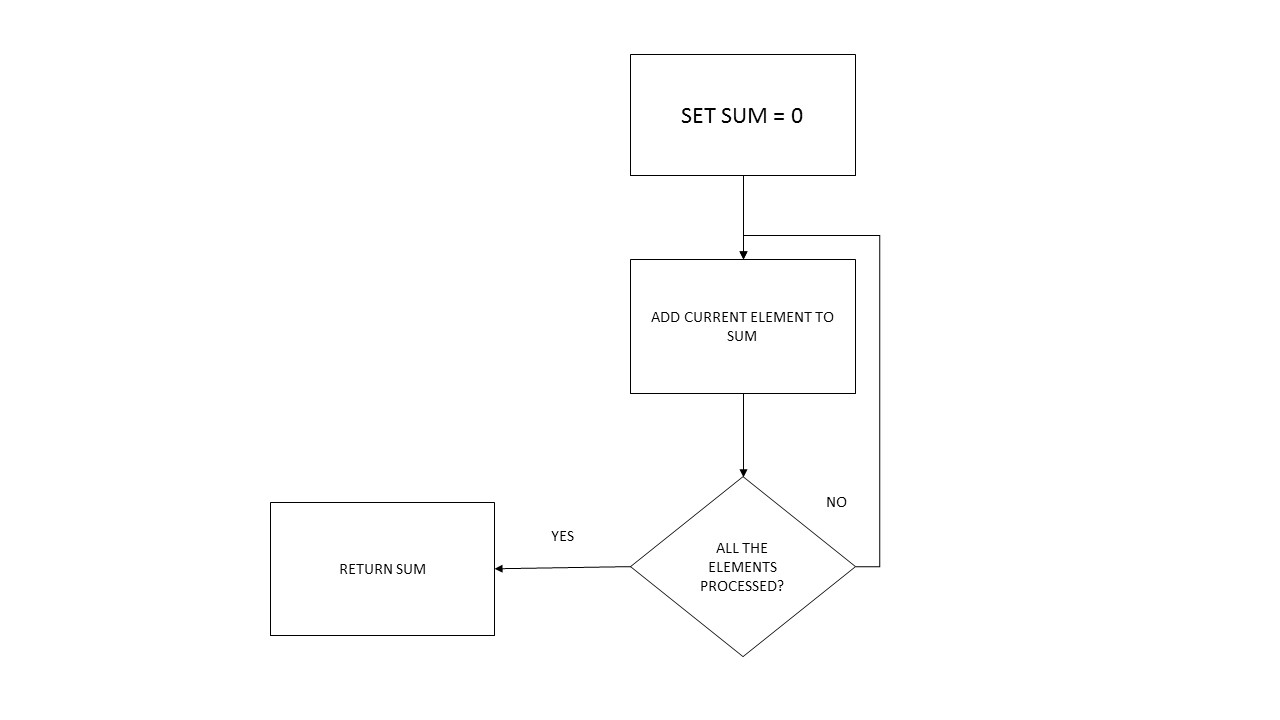
\includegraphics[width = \textwidth]{Figures/flow_chart}
	\caption{Flow chart for the sum of a sequence of numbers}
	\label{fig:ch1_flow_chart}
\end{figure}

\subsubsection*{Pseudocode}
Pseudocode is a semi-formal language that might contain also statements expressed in natural language and omits system specific code like opening file writers, printing messages on the standard output, or even some data structure declaration and initialization. It is intended mainly for human reading rather than machine reading. The pseudocode to sum a sequence of numbers is shown in Algorithm \ref{alg:ch1_pseudocode}.

\begin{algorithm}
	\caption{Pseudocode to perform the sum of a sequence of integer numbers}
	\label{alg:ch1_pseudocode}
	\begin{algorithmic}
		\Function{SumIntegers}{$l \text{ list of integers}$}
			\State $sum \gets 0$
			\ForAll {$x \text{ in } l$}
				\State $sum \gets sum + x$
			\EndFor
			\State \Return $sum$
		\EndFunction
	\end{algorithmic}
\end{algorithm}

\subsubsection*{Advantages and disadvantages}
Using flow charts or pseudo-code has the advantage of being able to define an algorithm in a way which is very close to the abstractions employed when using natural language: a flow chart combines both the use of natural language and a visual interface to describe an algorithm, pseudo-code allows to employ several abstractions and even define some steps in terms of natural language. The drawback of these two formal representations is that, when it comes to the implementation, the definition of the algorithm must be translated by hand into code that the hardware is able to execute. This could be done by implementing the algorithm in a low-level or high-level programming language. This process affects at different levels how the logic of the algorithm is presented, as explained further.

\section{Programming languages}
\label{sec:ch1_programming_languages}
A programming language is a formal language that is used to define instructions that a machine, usually a computer, must perform in order to produce a result through computation \cite{mordechai1996, narasimhan1967programming, oxford2008}. There is a wide taxonomy used to classify programming languages depending on their use \cite{kelleher2005lowering, myers1986visual, myers1990taxonomies}, but all can be grouped according to two main characteristics: the level of abstraction, or how close to the specific targeted hardware they are, and the domain, which defines the range of applicability of a programming language. In the following sections we give an exhaustive explanation of the aforementioned characteristics.

\subsection{Low-level programming languages}
\label{subsec:ch1_ll_languages}
A low-level programming language is a programming language that provides little to no abstraction from the hardware architecture of a processor. This means that it is strongly connected with the instruction set of the targeted machine, the set of instructions a processor is able to execute. These languages are divided into two sub-categories: \textit{first-generation} and \textit{second-generation} languages:

\subsubsection*{First-generation languages}
\textit{Machine code} falls into the category of first-generation languages. In this category we find all those languages that do not require code transformations to be executed by the processor. These languages were used mainly during the dawn of computer age and are rarely employed by programmers nowadays. Machine code is made of stream of binary data, that represents the instruction codes and their arguments \cite{guide2011intel, seal2001arm}. Usually this stream of data is treated by programmers in hexadecimal format, which is then remapped into binary code. The programs written in machine code were once loaded into the processor through a front panel, a controller that allowed the display and alteration of the registers and memory (see Figure \ref{fig:ch1_front_panel}). An example of machine code for a program that computes the sum of a sequence of integer numbers can be seen in Listing \ref{lst:ch1_machine_code}.

\begin{figure}
	\centering
	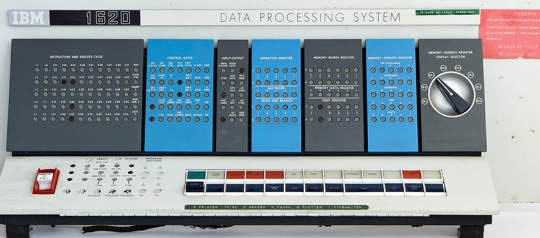
\includegraphics[width = \textwidth]{Figures/ch1_front_panel}
	\caption{Front panel of IBM 1620}
	\label{fig:ch1_front_panel}
\end{figure}

\begin{minipage}{\linewidth}
\begin{lstlisting}[numbers = left, caption = Machine code to compute the sum of a sequence of numbers, label = lst:ch1_machine_code]
 00075	c7 45 b8 00 00
 00 00
 0007c	eb 09	
 0007e	8b 45 b8
 00081	83 c0 01
 00084	89 45 b8
 00087	83 7d b8 0a
 0008b	7d 0f
 0008d	8b 45 b8
 00090	8b 4d c4
 00093	03 4c 85 d0
 00097	89 4d c4
 0009a	eb e2
\end{lstlisting}
\end{minipage}

\subsubsection*{Second-generation languages}
The languages in this category provides an abstraction layer over the machine code by expressing processor instructions with mnemonic names both for the instruction code and the arguments. For example, the arithmetic sum instruction \texttt{add} is the mnemonic name for the instruction code \texttt{0x00} in \texttt{x86} processors. Among these languages we find \textit{Assembly}, that is mapped with an \textit{Assembler} to machine code. The Assembler can load directly the code or link different \textit{object files} to generate a single executable by using a \textit{linker}. An example of assembly \texttt{x86} code corresponding to the machine code in Listing \ref{lst:ch1_machine_code} can be found in Listing \ref{lst:ch1_assembly_code}. You can see that the code in the machine code \texttt{00081	83 c0 01} at line 5 has been replaced by its mnemonic representation in Assembly as \texttt{add	eax, 1}.

\begin{minipage}{\linewidth}
\begin{lstlisting}[numbers = left, caption = Assembly x86 code to compute the sum of a sequence of numbers, label = lst:ch1_assembly_code]
mov	DWORD PTR _i$1[ebp], 0
jmp	SHORT $LN4@main
$LN2@main:
mov	eax, DWORD PTR _i$1[ebp]
add	eax, 1
mov	DWORD PTR _i$1[ebp], eax
$LN4@main:
cmp	DWORD PTR _i$1[ebp], 10			; 0000000aH
jge	SHORT $LN3@main
mov	eax, DWORD PTR _i$1[ebp]
mov	ecx, DWORD PTR _sum$[ebp]
add	ecx, DWORD PTR _numbers$[ebp+eax*4]
mov	DWORD PTR _sum$[ebp], ecx
jmp	SHORT $LN2@main
\end{lstlisting}
\end{minipage}

\subsubsection*{Advantages and disadvantages}
Writing a program in low-level programming languages might produce programs that are generally more efficient than their high-level counterparts, as ad-hoc optimizations are possible. However, the high-performance comes at great costs: (\textit{i}) the programmer must be an expert of the underlying architecture and of the specific instruction set of the processor, (\textit{ii}) the program loses portability because the low-level code is tightly bound to the specific hardware architecture it targets, (\textit{iii}) the logic and readability of the program is hidden among the details of the instruction set itself, and (\textit{iv}) developing a program in assembly requires a considerable effort in terms of time and debugging \cite{frampton2009demystifying}: assembly lacks any abstraction from the concrete hardware architecture, such as a type system, that partially ensures the correctness of the program or high-level constructs that allow to manipulate the execution of the program.

\subsection{High-level programming languages}
\label{subsec:ch1_hl_languages}
A high-level programming language is a programming language that offers a high level of abstraction from the specific hardware architecture of the machine. Unlike machine code (and in some way also assembly), high-level languages are not directly executable by the processor and they require some kind of translation process into machine code. The level of abstraction offered by the language defines how high level the language is. Several categories of high-level programming language exist, but the main one are described below.

\subsubsection*{Imperative programming languages}
\textit{Imperative programming languages} model the computation as a sequence of statements that alter the state of the program (usually the memory state). A program in such languages consists then of a sequence of \textit{commands}. Notable examples are FORTRAN, C, and PASCAL. An example of the program used in Listing \ref{lst:ch1_machine_code} and \ref{lst:ch1_assembly_code} written in C can be seen in Listing \ref{lst:ch1_c_code}. Line 5 to 9 corresponds to the Assembly code in Listing \ref{lst:ch1_assembly_code}.

\begin{lstlisting}[numbers = left, caption = C code to compute the sum of a sequence of numbers, label = lst:ch1_c_code]
int main()
{
  int numbers[10] = { 1, 6, 8, -2, 4, 3, 0, 1, 10, -5 };
  int sum = 0;
  for (int i = 0; i < 10; i++)
  {
    sum += numbers[i];
  }
  printf("%d\n", sum);
}
\end{lstlisting}

\subsection*{Declarative programming languages}
\textit{Declarative programming languages} are antithetical to those based on imperative programming, as they model computation as an evaluation of expressions and not as a sequence of commands to execute. Declarative programming languages are called as such when they are side-effects free or referentially transparent. The definition of referential transparency varies \cite{quine2013word}, but it is usually explained with the substitution principle, which states that a language is referentially transparent if any expression can be replaced by its value without altering the behaviour of the program \cite{mitchell2003concepts}. For instance, the following sentences in natural language are both true

\begin{lstlisting}
Cicero = Tullius

''Cicero`` contains six letters
\end{lstlisting} 

\noindent
but they are not referentially transparent, since replacing the last name with the middle name falsifies the second sentence.

A similar situation in programming languages is met when considering variable assignments: the statement

\begin{lstlisting}
x = x + 5
\end{lstlisting}

\noindent
is not referentially transparent. Let us assume this statement appears twice in a program and that at the beginning x = 0. Clearly the expression \texttt{x + 5} results in the value 5 the first time, but the second time the same statement is executed the expression has value 10. Thus replacing all the occurrences of \texttt{x + 5} with 5 is wrong, which is why imperative languages are not referentially transparent. A more rigorous definition of referential transparency can be found in \cite{sondergaard1990referential}.

Declarative programming languages are often compared to imperative programming languages by stating that declarative programming defines \textit{what} to compute and not \textit{how} to compute it. This family of languages include \textit{functional programming}, \textit{logic programming}, and \textit{database query languages}. Notable examples are F\#, Haskell, Prolog, SQL, and Linq (which is a query language embedded in C\#). Listing \ref{lst:ch1_fsharp_code_rec} shows the code to perform the sum of a sequence of integer numbers in F\# with a recursive function. Higher-order functions, such as \texttt{fold}, allow even to capture the same recursive pattern into a single function as shown in Listing \ref{lst:ch1_fsharp_code_fold}. Both implementations are referentially transparent.

\begin{lstlisting}[caption = Recursive F\# code to compute the sum of a sequence of numbers, label = lst:ch1_fsharp_code_rec]
let rec sumList l =
  match l with
  | [] -> 0
  | x :: xs -> x + (sumList xs)
\end{lstlisting}

\begin{lstlisting}[caption = F\# code to compute the sum of a sequence of numbers using higher-order functions, label = lst:ch1_fsharp_code_fold]
let sumList l = l |> List.fold (+) 0
\end{lstlisting}

\subsection{General-purpose vs Domain-specific languages}
\label{sec:ch1_dsl}
\textit{General-purpose languages} are defined as languages that can be used across different application domains and lack abstractions that specifically target elements of a single domain. Example of these are languages such as C, C++, C\#, and Java. Although several applications are still being developed by using general-purpose programming languages, in several contexts it is more convenient to rely on \textit{domain-specific languages}, because they offer abstractions relative to the problem domain that are unavailable in general-purpose languages \cite{van2000domain, voelter2013dsl}. Notable examples of the use of domain-specific languages are listed below.

\subsubsection*{Graphics programming}
Rendering a scene in a 3D space is often performed by relying on dedicated hardware. Modern graphics processors rely on shaders to create various effects that are rendered in the 3D scene. Shaders are written in domain-specific languages, such as GLSL or HLSL \cite{glhl2014, hlsl2018, hlslref2018}, that offer abstractions to compute operations at GPU level that are often used in computer graphics, such as vertices and pixel transformations, matrix multiplications, and interpolation of textures. Listing \ref{lst:ch1_hlsl_code} shows the code to implement light reflections in HLSL. At line 4 you can, for example, see the use of matrix multiplication provided as a language abstraction in HLSL.

\begin{lstlisting}[numbers = left, caption = HLSL code to compute the light reflection, label = lst:ch1_hlsl_code]
VertexShaderOutput VertexShaderSpecularFunction(VertexShaderInput input, float3 Normal : NORMAL)
{
  VertexShaderOutput output;
  float4 worldPosition = mul(input.Position, World);
  float4 viewPosition = mul(worldPosition, View);
  output.Position = mul(viewPosition, Projection);
  float3 normal = normalize(mul(Normal, World));
  output.Normal = normal;
  output.View = normalize(float4(EyePosition,1.0f) - worldPosition);
  return output;
}
\end{lstlisting}

\subsubsection*{Game programming}
Computer games are a field where domain-specific languages are widely employed, as they contain complex behaviours that often require special constructs to model timing event-based primitives, or to execute tasks in parallel. These behaviours cannot be modelled, for performance reasons, by using threads. Therefore, in the past, domain-specific languages which provide these abstractions have been implemented \cite{nwnlexicon2018, jass2011, unrealscript2018, sqf2018}. In Listing \ref{lst:ch1_sqf_code} an example of the SQF domain-specific language for the game ArmA2 is shown. This language offers abstractions to wait for a specific amount of time, to wait for a condition, and to spawn scripts that run in parallel to the callee, that you can respectively see at lines 18, 12, and 10.

\begin{lstlisting}[numbers = left, caption = ArmA 2 scripting language, label = lst:ch1_sqf_code]
"colorCorrections" ppEffectAdjust [1, pi, 0, [0.0, 0.0, 0.0, 0.0], [0.05, 0.18, 0.45, 0.5], [0.5, 0.5, 0.5, 0.0]];  
"colorCorrections" ppEffectCommit 0;  
"colorCorrections" ppEffectEnable true;

thanatos switchMove "AmovPpneMstpSrasWrflDnon";
[[],(position tower) nearestObject 6540,[["USMC_Soldier",west]],4,true,[]] execVM "patrolBuilding.sqf";
playMusic "Intro";

titleCut ["", "BLACK FADED", 999];
[] Spawn 
{
	waitUntil{!(isNil "BIS_fnc_init")};
	[
	  localize "STR_TITLE_LOCATION" ,
	  localize "STR_TITLE_PERSON",
	  str(date select 1) + "." + str(date select 2) + "." + str(date select 0)
	] spawn BIS_fnc_infoText;
	sleep 3;
	"dynamicBlur" ppEffectEnable true;   
	"dynamicBlur" ppEffectAdjust [6];   
	"dynamicBlur" ppEffectCommit 0;     
	"dynamicBlur" ppEffectAdjust [0.0];  
	"dynamicBlur" ppEffectCommit 7;
	titleCut ["", "BLACK IN", 5];
};
\end{lstlisting}

\subsubsection*{Shell scripting languages}
Shell scripting languages, such as the \textit{Unix Shell script}, are used to manipulate files or user input in different ways. They generally offer abstractions to the operating system interface in the form of dedicated commands. Listing \ref{lst:ch1_shell_code} shows an example of a program written in Unix shell script to convert an image from JPG to PNG format. At line 3 you can see the use of the statement \texttt{echo} to display a message in the standard output.

\begin{lstlisting}[numbers = left, caption = Unix shell code, label = lst:ch1_shell_code]
for jpg; do                                  
  png="${jpg%.jpg}.png"                    
  echo converting "$jpg" ...               
  if convert "$jpg" jpg.to.png ; then      
    mv jpg.to.png "$png"                 
  else                                     
    echo 'jpg2png: error: failed output saved in "jpg.to.png".' >&2
    exit 1
  fi                                       
done                                         
echo all conversions successful              
exit 0
\end{lstlisting}

\subsubsection*{Advantages and disadvantages}
High-level programming languages offer a variety of abstractions over the specific hardware the program targets. The obvious advantage of this is that the programmer does not need to be an expert of the underlying hardware architecture or instruction set. A further advantage is that the available abstractions are closer to the semi-formal description of the underlying algorithm as pseudo-code. This produces two desirable effects: (\textit{i}) the readability of the program is increased as the available abstractions are closer to the natural language than the equivalent machine code, and (\textit{ii}) that being able to mimic the semi-formal version of an algorithm, which is generally how the algorithm is presented and on which its correctness is proven, grants a higher degree of correctness in the specific implementation.

The use of a high-level programming language might, in general, not achieve the same high-performance as writing the same program with a low-level programming language  \cite{chatzigeorgiou2002evaluating}, but modern code-generation optimization techniques can generally mitigate this gap \cite{amarasinghe1993communication, wang2007code}. A further major issue in using high-level programming languages is that the machine cannot directly execute the code, thus the use of a compiler that translates the high-level program into machine code is necessary.

The portability of a high-level programming language depends on the architecture of the underlying compiler, thus some languages are portable and the same code can be run on different machines (for example Java), while others might require to be compiled to target a specific architecture (for example C++).

\section{Compilers}
\label{sec:ch1_compilers}
A compiler is a program that transforms source code defined in a programming language into another computer language, which usually is object code but can also be code in a high-level programming language \cite{aho2007compilers, appel2002javacompiler}. Writing a compiler is a necessary step to implementing a high-level programming language. Indeed, a high-level programming language, unlike low-level ones, are not executable directly by the processor and need to be translated into machine code, as stated in Section \ref{subsec:ch1_ll_languages} and \ref{subsec:ch1_hl_languages}.

The first complete compiler was developed by IBM for the FORTRAN language and required 18 person-years for its development \cite{backus1957fortran}. This clearly shows that writing a compiler is a hard and time-consuming task.

A compiler is a complex piece of software made of several components that implement a step in the translation process. The translation process performed by a compiler involves the following steps:

\begin{enumerate}
	\item \textit{syntactical analysis:} In this phase the compiler checks that the program is written according to the grammar rules of the language. In this phase the compiler must be able to recognize the \textit{syntagms} of the language (the ``words'') and also check if the program conforms to the syntax rules of the language through a grammar specification.
	\item \textit{type checking:} In this phase the compiler checks that a \textit{syntactically correct program} performs operations conform to a defined \textit{type system}. A type system is a set of rules that assign properties called types to the constructs of a computer program \cite{pierce2002types}. The use of a type system drastically reduces the chance of having bugs in a computer program \cite{cardelli1996type} . This phase can be performed at compile time (\textit{static typing}) or the generated code could contain the code to perform the type checking at runtime (\textit{dynamic typing}). 
	\item \textit{code generation:} In this phase the compiler takes the \textit{syntactically and type-correct program} and performs the translation step. At this point an equivalent program in a target language will be generated. The target language can be object code, another high-level programming language, or even a bytecode that can be interpreted by a virtual machine.
\end{enumerate}

All the previous steps are always the same regardless of the language the compiler translates from and they are not part of the creative aspect of the language design \cite{book1970cwic}. Approaches to automating the construction of the syntactical analyser are well known in literature \cite{mcpeak2004elkhound, nivre2006maltparser, parr1995antlr}, to the point that several lexer/parser generators are available for programmers, for example all those belonging to the \texttt{yacc} family such as \texttt{yacc} for C/C++, \texttt{fsyacc} for F\#, \texttt{cup} for Java, and \texttt{Happy} for Haskell. On the other hand, developers lack a set of tools to automate the implementation of the last two steps, namely the type checking and the code generation.

For this reason, when implementing a compiler, the formal type system definition and the operational semantics, which is tightly connected to the code generation and defines how the constructs of the language behave, must be translated into the abstractions provided by the host language in which the compiler will be implemented. Other than being a time-consuming activity itself, this causes that (\textit{i}) the logic of the type system and operational semantics is lost inside the abstraction of the host-language, and (\textit{ii}) it is difficult to extend the language with new features.

\section{Meta-compilers}
\label{sec:ch1_metacompilers}
In Section \ref{sec:ch1_compilers} we described how the steps involved in designing and implementing a compiler do not require creativity and are always the same, regardless of the language the compiler is built for. The first step, namely the syntactical analysis, can be automated by using one of the several lexer/parser generators available, but the implementation of a type checker and a code generator still relies on a manual implementation. This is where meta-compilers come into play: a meta-compiler is a program that takes the source code of another program written in a specific language and the language definition itself, and generates executable code. The language definition is written in a programming language, referred to as \textit{meta-language}, which should provide the abstractions necessary to define the syntax, type system, and operational semantics of the language, in order to implement all the steps above.

\subsection{Requirements}
As stated in Section \ref{sec:ch1_metacompilers}, a meta-compiler should provide a meta-language that is able to define the syntax, type system, and operational semantics of a programming language. In Section \ref{sec:ch1_compilers} we discussed how methods to automate the implementation of syntactical analyser are already known in scientific literature. For this reason, in this work, we will focus exclusively on automating the implementation of the type system and of the operational semantics. Given this focus, we formulate the following requirements:

\begin{itemize}
	\item The meta-language should provide abstractions to define the constructs of the language. This includes the possibility of defining control structures, operators with any form of prefix or infix notation, and the priority of the constructs that is used when evaluating their behaviour. Furthermore, it must be possible to define the equivalence of language constructs. For instance, an integer constant might be considered both a value and a basic arithmetic expression.
	
	\item The meta-language must be able to mimic as close as possible the formal definition of a programming language. This will bring the following benefits: (\textit{i}) Implementing the language in the meta-compiler will just involve re-writing almost one-to-one the type system or the semantics of the language with little or no change; (\textit{ii}) the correctness and soundness \cite{cardelli1996type, milner1972proving} of the language formal definition will be directly reflected in the implementation of the language; indeed if a meta-program allows to mimic directly the type system and semantics of the language their correctness is transferred also in the implementation, while this might not be trivial when translating them in the abstractions of a high-level programming language; (\textit{iii}) any extension of the language definition can be just added as an additional rule in the type system or the semantics.
	
	\item The meta-compiler must be able to embed libraries from external languages, so that they can be used to implement specific behaviours such as networking transmission or specific data structure usage.
\end{itemize}

\subsection{Benefits}
\label{sec:ch1_benefits}
%list the benefits first and then explain. Add a paragraph also about correctness
Programming languages usually are released with a minimal (but sufficient to be Turing-complete) set of features, and later extended in functionality in successive versions. This process tends to be slow and often significant improvements or additions are only seen years after the first release. For example, Java was released in 1996 and lacked an important feature such as Generics until 2004, when J2SE 5.0 was released. Furthermore, Java and C++ lacked constructs from functional programming, which is becoming more and more popular with the years \cite{thompson1995miranda}, such as lambda abstractions until 2016, while a similar language like C\# 3.0 was released with such capability in 2008. The slow rate of change of programming languages is due to the fact that every abstraction added to the language must be reflected in all the modules of its compiler: the grammar must be extended to support new syntactical rules, the type checking of the new constructs must be added, and the appropriate code generation must be implemented. Given the complexity of compilers, this process requires a huge amount of work, and it is often obstructed by the low flexiblity of the compiler as piece of software. Using a meta-compiler would speed up the extension of an existing language because it would require only to change on paper the type system and the operational semantics, and then add the new definitions to their counterpart written in the meta-language. This process is easier because the meta-language should mimic as close as possible their behaviour. Moreover, backward compatibility is automatically granted because an older program will simply use the extended language version to be compiled by the meta-compiler.

To this we add the fact that, in general, for the same reasons, the development of a new programming language is generally faster when using a meta-compiler. This could be beneficial to the development of a high variety of domain-specific languages. Indeed, such languages are often employed in situations where the developers have little or no resources to develop a fully-fledged hard-coded compiler by hand. For instance, it is desirable for game developers to focus on aspects that are strictly tied to the game itself, for example the development of an efficient graphics engine or to improve the game logic. At the same time they would need a domain-specific language to express some behaviours typical of games, things that could be achieved by using a meta-compiler rather than on a hand-made implementation.

\subsection{Scientific relevance} %change the tile
\label{sec:ch1_scientific_relevance}
Meta-compilers have been researched since the 1960's \cite{schorre1964meta} and several implementations have been proposed \cite{ braborovansky1998overview, venboer2008stratego, klint2009rascal, pettersson1996compiler, verdejo2006executable}. In general meta-compilers perform poorly compared to hard-coded compilers because they add the additional layer of abstraction of the meta-language. Moreover, a specific implementation of a compiler opens up the possibility of implementing language-specific optimizations during the code generation phase. Meta-compilers have been used in a wide range of applications, such as source code analysis and manipulation and physical simulations \cite{kaagedal1998generating}, but no use up to our knowledge was made in the field of domain-specific languages for games. Since games are pieces of software that are very demanding in terms of performance, we think that it could be of interest to investigate the applicability of meta-compilers in the scope of domain-specific languages for games and the development speed up introduced by the use of such a tool. In this work we present Metacasanova, a meta-compiler based on natural semantics that was born from the intent of easing the development of the domain-specific language for game development Casanova, and we analyse the benefit of using it for a re-implementation and extension of Casanova.

\section{Problem statement}
\label{sec:ch1_problem_statement}
In Section \ref{sec:ch1_programming_languages} we showed the advantages of using high-level programming languages when implementing an algorithm. Among such languages, it is sometimes desirable to employ domain-specific languages that offer abstractions relative to a specific application domain (Section \ref{sec:ch1_dsl}). In Section \ref{sec:ch1_compilers} we described the need of a compiler for such languages, and that developing one is a time-consuming activity despite the process being, in great part, non-creative. In Section \ref{sec:ch1_metacompilers} we introduced the role of meta-compilers to speed up the process of developing a compiler and we listed the requirements and the benefits that one should have. In Section \ref{sec:ch1_scientific_relevance} we explained why we believe that meta-compilers are a relevant scientific topic if coupled with the problem of of developing domain-specific languages in response to the their increasing need. We can now formulate our problem statement:

\vspace{0.5cm}
\noindent
\textbf{Problem statement: } \textit{\psContent}

\vspace{0.5cm}
\noindent
The first parameter we need to evaluate in order to answer this question is the size of the code reduction needed to implement the domain-specific language. At this purpose, the following research question arises:

\vspace{0.5cm}
\noindent
\textbf{Research question 1: } \textit{\rqContentOne}

\vspace{0.5cm}
\noindent
The second parameter we need to evaluate is the eventual performance loss caused by introducing the abstraction layer provided by the meta-compiler. This leads to the following research question:

\vspace{0.5cm}
\noindent
\textbf{Research question 2: } \textit{\rqContentTwo}

\vspace{0.5cm}
\noindent
In case of a performance loss, we need to identify the cause of this performance loss and if an improvement is possible. This leads to the following research question:

\vspace{0.5cm}
\noindent
\textbf{Research question 3: } \textit{\rqContentThree}

\vspace{0.5cm}
\noindent

\section{Thesis structure}
This thesis describes the architecture of Metacasanova, a meta-compiler whose meta-language is based on operational semantics, and a possible optimization for such meta-compiler. It also shows its the capabilities by implementing a small imperative language and re-implementing the existing domain-specific language for games \textit{Casanova 2}, extending it with abstractions to express network operations for multiplayer games.

In Chapter \ref{ch:background} we provide background information in order to understand the choices made for this work. The chapter presents the state of the art in designing and implementing compilers and existing research on meta-compilers.

In Chapter \ref{ch:metacasanova} we present the architecture of Metacasanova by extensively describing the implementation of all its modules.

In Chapter \ref{ch:languages} we show how to use Metacasanova to implement two languages: a small imperative language, and \textit{Casanova 2}, a language for game development. At the end of the chapter we provide an evaluation of the performance of the two languages and their implementation length with respect to existing compilers, thus answering to Research Question 1 and 2.

In Chapter \ref{ch:functors} we discuss the performance loss of the implementation of the presented languages and we propose an extension of Metacasanova that aims to improve the performance of the generated code, thus answering Research Question 3.

In Chapter \ref{ch:functor_languages} we show how to use functors to improve the performance of Casanova implemented in Metacasanova, comparing this approach and the one presented in Chapter \ref{ch:languages} with respect to the execution time of a sample in Casanova. 

In Chapter \ref{ch:networking} we propose an extension of Casanova 2 for multiplayer game development. We first provide its hard-coded compiler solution and then we show how to extend the implementation in the meta-compiler to include the same extension. In this chapter we evaluate the performance of a multiplayer game implemented in Casanova with this extension with respect to the same game implemented in C\#, and we measure the effort of realising such extension in the hard-coded compiler of Casanova versus the implementation with Metacasanova.

In Chapter \ref{ch:discussion} we discuss the result and answer the research questions.

\section{Repetitive steps in compilers development}
\label{sec:problem}
Within the context of higher education, learning programming is hard for both beginners and students with past experience. 

It is suggested by some \cite{tan2009learning} that learning programming is no different than most other complex skills: it takes roughly ten years (ten thousand hours) to become truly proficient.

The reason why it takes so long is disarmingly simple. Programming requires both the ability to \textit{understand} and to \textit{design} code. 

\subsection{Understanding code}
Understanding code is a passive skill, but not any simpler because of it. The true meaning of code is the sequence of steps that the machine will actually perform: every single bit that will be read and written as a result of an instruction is part of the meaning of that instruction, just like every cache hit-or-miss, the activation of the CPU ALU(s), network channels, operating systems, interpreters, just-in-time compilers, and ultimately interactions with users. Being able to figure precisely what a program does, and how it does it (also in terms of performance) requires the ability to formulate an abstract idea of the program behaviour, and the mapping of this \textit{abstract idea} to the concrete components when more specific reasoning is needed.

The sheer size of the machinery involved in the execution of even the simplest program is simply \textit{very large}, and \textit{the ability to think hierarchically and zoom in and out of the details as needed takes a lot of experience}.

\subsection{Designing code}
Designing code is an active skill, and as such intrinsically complex. Designing code requires the formulation (and therefore the choice) of a design strategy, usually in a top-down fashion, which is then recursively turned into a more and more concrete definition of the program. Being able to design a program effectively requires the ability to choose a specific design among a series of possible designs, which taken together form \textit{the abstract meta-strategies} that characterise a programmer’s knowledge, style, and experience.

The sheer size of the design space of even the simples program is \textit{so large as to be essentially infinite} (we are talking about finite machines after all!), and the ability to \textit{formulate meta-strategies and employ them recursively takes a lot of experience}.

\subsection{Size matters (and so does structure)}
We believe the size of the domain to be the core of the issue. Even though some students might already know a few tricks to produce working programs in some very narrow domain, the fundamental ability to abstractly reason about code (both for understanding and designing programs) is usually severely lacking in first year students.

Moreover, we cannot just solve the problem by throwing unstructured assignments such as “read this code” or “try and write this program”, as we must train the specific mental activities that we wish to stimulate in students. Specific training must be structured in order to gently guide the activation of the proper thought structures, in a slow buildup of complexity and freedom to express one’s own creativity.

\subsection{The issues}
We close this session by identifying a series of practical, concrete issues that we believe sum up the discussion so far:

\begin{table}[!h]
	\begin{tabular}{|c|p{8cm}|}
		\hline
		\textbf{ID} & \textbf{Issue} \\
		\hline
		REASON\textunderscore MODEL & Students need extensive practice with reasoning about models of programs \\
		\hline
		REASON\textunderscore DESIGN & Students need extensive practice with reasoning about existing design strategies \\
		\hline
		EXTEND\textunderscore DESIGN & Students need extensive practice with extending existing programs (which should follow a formative design). \\
		\hline
		EXTEND\textunderscore BUILDUP & Students need a buildup in complexity with their extension activities. \\
		\hline
	\end{tabular}
	\caption{Issues about learning programming}
	\label{tab:issues}
\end{table}

By keeping these issues in mind, we will now setup a proposed didactic model which we believe can mitigate them or outright resolve them.





\section{Metacasanova syntax and semantics}
\label{sec:semantics}
In the previous section we showed that the process of evaluating typing and semantics rules is always the same, regardless of the specific language implementation. We have also discussed how this evaluation must be re-implemented every time in a hard-coded compiler by using the abstractions provided by the host language, which leads to verbose code and the loss of the clarity and simplicity given by the formalisms of the type system and operational semantics. In this section we define the requirements of Metacasanova, we informally present, through an example, how a meta-program works, and we finally propose the syntax and semantics of its meta-language.

\subsection{Requirements of Metacasanova}
In order to relieve programmers of manually defining the behaviour described in Section \ref{sec:problem} in the back-end of the compiler, we propose the following features for Metacasanova:

\begin{itemize}
	\item It must be possible to define custom operators (or functions) and data containers. This is needed to define the syntactic structures of the language we are defining.
	\item It must be typed: each syntactic structure can be associated to a specific type in order to be able to detect meaningless terms (such as adding a string to an integer) and notify the error.
	\item It must be possible to have polymorphic syntactical structures. This is useful to define equivalent ``roles'' in the language for the same syntactical structure; for instance we can say that an integer literal is both a \textit{Value} and an \textit{Arithmetic expression}.
	\item It must natively support the evaluation of semantics rules, as those shown above. A \textit{rule},in Metacasanova, in the fashion of a logic rule, is made of a sequence of premises and a conclusion. The premises can be function calls or clauses. Clauses are boolean expressions that are checked in order to proceed with the rule evaluation. The function call will run in order all the rules that contain that function as conclusion. The return value of the first rule that succeeds is taken. A rule returns a value if all the clauses evaluate to \texttt{true} and all the function calls succeed.
\end{itemize}

We can see that these specifications are compatible with the definition of meta-compiler, as the software takes as input a language definition written in the meta-language, a program for that language, and outputs runnable code that mimics the code that a hard-coded compiler would output.

\subsection{General overview}

A Metacasanova program is made of a set of \texttt{Data} and \texttt{Function} definitions, and a sequence of rules. A data definition specifies the constructor name of the data type (used to construct the data type), its field types, and the type name of the data. Optionally it is possible to specify a priority for the constructor of the data type. For instance this is the definition of the sum of two arithmetic expression

\begin{lstlisting}
Data Expr -> "+" -> Expr : Expr  Priority 500
\end{lstlisting}

\noindent
Note that Metacasanova allows you to specify any kind of notation for data types in the language syntax, depending on the order of definition of the argument types and the constructor name. In the previous example we used an infix notation. The equivalent prefix and postfix notations would be:

\begin{lstlisting}
Data "+" -> Expr -> Expr : Expr
Data Expr -> Expr -> "+" : Expr
\end{lstlisting}

\noindent
A function definition is similar to a data definition but it also has a return type. For instance the following is the evaluation function definition for the arithmetic expression above:

\begin{lstlisting}
Func "eval" -> Expr : Evaluator => Value
\end{lstlisting}

\noindent
In Metacasanova it is also possible to define polymorphic data in the following way:

\begin{lstlisting}
Value is Expr
\end{lstlisting}

\noindent
In this way we are saying that an atomic value is also an expression and we can pass both a composite expression and an atomic value to the evaluation function defined above.

Metacasanova also allows to embed C\# code into the language by using double angular brackets. This code can be used to embed .NET types when defining data or functions, or to run C\# code in the rules. For example in the following snippets we define a floating point data which encapsulates a floating point number of .NET to be used for arithmetic computations:

\begin{lstlisting}
Data "$f" -> <<float>> : Value
\end{lstlisting}

\noindent
A rule in Metacasanova, as explained above, may contain a sequence of function calls and clauses. In the following snippet we have the rule to evaluate the sum of two floating point numbers:

\begin{lstlisting}
eval a => $f c
eval b => $f d
<<c + d>> => res
------------------------
eval (a + b) => $f res
\end{lstlisting}

\noindent
Note that if one of the two expressions does not return a floating point value, then the entire rule evaluation fails. Also note that we can embed C\# code to perform the actual arithmetic operation. Metacasanova selects a rule by means of pattern matching in order of declaration on the function arguments. This means that both of the following rules will be valid candidates to evaluate the sum of two expressions:

\begin{lstlisting}
...
---------------
eval expr => res

...
----------------
eval (a + b) => res
\end{lstlisting} 

Finally the language supports expression bindings with the following syntax:

\begin{lstlisting}
x := $f 5
\end{lstlisting}

\subsection{Syntax in BNF}
The following is the syntax of Metacasanova in Backus-Naur form. Note that, for brevity, we omit the definitions of typical syntactical elements of programming languages, such as literals or identifiers:

\begin{lstlisting}
<program> ::= 
{<include>} {<import>} {<data>} <function> {<function>} {<alias>} <rule> {<rule>}
<premise> ::= 
<clause> | <functionCall> | <binding>
<binding> ::= 
id ":=" <constructor>
<rule> ::= 
{premise} "-" {"-"} <functionCall>
<clause> ::= //typical boolean expression
<functionCall> ::= 
<id> {<argument>} <arrow> <argument> | 
{<argument>} <id> {<argument>} <arrow> <argument> | 
<id> {<argument>} <arrow> <argument>
<arrow> ::= "=>" | "==>"
<constructor> ::= 
<id> {<argument>} | 
{<argument>} <id> {<argument>} | 
{<argument>} <id>
<external> ::= "<<" <csharpexpr> ">>"
<csharpexpr> ::= //all available C# expressions
<argument> ::= 
["("] 
(<id> | 
<external> | 
<literal> | 
<constructor>) 
[")"]
<literal> ::= //typical literals such as integer, float, string, ...
<import> ::= import id {"." id}
<include> ::= include id {.id}
<alias> ::= <typeDef> is <typeDef>
<typeDef> ::= id | "<<" id ">>"
<typeArguments> :: = 
'"' <id> '"' {"->" <typeDef>} ":" <typeDef> |
<typeDef> {"->" <typeDef>} "->" '"' <id> '"' {"->" <typeDef>} ":" <typeDef> |
<typeDef> {"->" typeDef} "->" '"' <id> '"' ":" <typeDef> 
<function> ::= Func <typeArguments> "=>" <typeDef> [Priority <literal>]
<data> ::= Data <typeArguments> [Priority <literal>]
\end{lstlisting}

\subsection{Semi-formal Semantics}
In what follows we assume that the pattern matching of the function arguments in a rule succeeds, otherwise a rule will fail to return a result.
The informal semantics of the rule evaluation in Metacasanova is the following:
\begin{enumerate}
	\item[R1] A rule with no clauses or function calls always returns a result.
	\item[R2] A rule returns a result if all the clauses evaluate to \texttt{true} and all the function calls in the premise return a result.
	\item[R3] A rule fails if at least one clause evaluates to \texttt{false} or one of the function calls fails (returning no results).
\end{enumerate}
We will express the semantics, as usual, in the form of logical rules, where the conclusion is obtained when all the premises are true.
In what follows we consider a set of rules defined in the Metacasanova language $R$. Each rule has a set of function calls $F$ and a set of clauses (boolean expressions) $C$. We use the notation $f^{r}$ to express the application of the function $f$ through the rule $r$. We will define the semantics by using the notation $\langle expr \rangle$ to mark the evaluation of an expression, for example $\langle f^{r} \rangle$ means evaluating the application of $f$ through $r$. Note that in R2 the evaluation returns a set of result because there might be more than one rule that can successfully evaluate the premise. The following is the formal semantics of the rule evaluation in Metacasanova, based on the informal rules defined above:


\begin{mathpar}
	\mprset{flushleft}
	\inferrule*[left=R1:]
	{C = \emptyset \\\\ F = \emptyset}
	{\langle f^{r} \rangle \Rightarrow x} \\
	
	\mprset{flushleft}
	\inferrule*[left=R2:]
	{\forall c_{i} \in C \;, \langle c_{i} \rangle \Rightarrow true \\\\
		\forall f_{j} \in F \; \exists r_{k} \in R \; | \; \langle f_{j}^{r_{k}} \rangle \Rightarrow \lbrace x_{k_{1}}, x_{k_{2}}, ..., x_{k_{m}} \rbrace}
	{\langle f^{r} \rangle \Rightarrow \lbrace x_{1}, x_{2}, ..., x_{n} \rbrace} \\
	
	\mprset{flushleft}
	\inferrule*[left=R3(a):]
	{\exists c_{i} \in C \; | \; \langle c_{i} \rangle \Rightarrow false}
	{\langle f^{r} \rangle \Rightarrow \emptyset} \\
	
	\mprset{flushleft}
	\inferrule*[left=R3(b)]
	{\forall r_{k} \in R \; \exists f_{j} \in F \; | \; \langle f_{j}^{r_{k}} \rangle \Rightarrow \emptyset}
	{\langle f^{r} \rangle \Rightarrow \emptyset}
\end{mathpar}

R1 says that, when both $C$ and $F$ are empty (we do not have any clauses or function calls), the rule in Metacasanova returns a result. R2 says that, if all the clauses in $C$ evaluates to true and, for all the function calls in $F$ we can find a rule that returns a result (all the function applications return a result for at least one rule of the program), then the current rules return a result. R3(a) and R3(b) specify when a rule fails to return a result: this happens when at least one of the clauses in $C$ evaluates to false, or when one of the function applications does not return a result for any of the rules defined in the program.

\vspace{0.2cm}
\noindent
In the following section we describe how the code generation process works, namely how the \texttt{Data} types of Metacasanova are mapped in the target language, and how the rule evaluation is implemented.

\section{Code generation}
\label{sec:code_generation}
In Section \ref{sec:semantics} we defined the syntax and semantics of Metacasanova. In this section we explain how the abstractions of the language are compiled into the generated code. We chose C\# as target language because the development of Metacasanova started with the idea of expanding the DSL for game development Casanova with further functionalities. Casanova hard-coded compiler generates C\# code as well because it is compatible with game engines such as Unity3D and Monogame. At the same time, C\# grants decent performance without having to manually manage the memory such as for lower-level languages like C/C++. Code generation in different target languages is possible but still an ongoing project (see Section \ref{sec:conclusion}).

\subsection{Data Structures Code Generation}
The type of each data structure is generated as an interface in C\#. Each data structure defined in Metacasanova is mapped to a \texttt{class} in C\# that implements such interface. The class contains as many fields as the number of arguments the data structure contains. Each field is given an automatic name \texttt{argC} where \texttt{C} is the index of the argument in the data structure definition. The data structure symbols used in the definition might be pre-processed and replaced in order to avoid illegal characters in the C\# class definition. The class contains an additional field that stores the original name of the data structure before the replacement is performed, used for its ``pretty print''. For example the data structure

\begin{lstlisting}
Data "$i" -> int : Value
\end{lstlisting}

\noindent
will be generated as

\begin{lstlisting}
public interface Value {  }

public class __opDollari : Value
{
  public string __name = "$i";
  public int __arg0;

  public override string ToString()
  {
    return "(" + __name + " " + __arg0 + ")";
  }
}
\end{lstlisting}

\subsection{Code Generation for Rules}
Each rule contains a set of premises that in general call different functions to produce a result, and a conclusion that contains the function evaluated by the current rule and the result it produces. The code generation for the rules follows the steps below:

\begin{enumerate}
	\item Generate a data structure for each function defined in the meta-program.
	\item For each function $f$ extract all the rules whose conclusion contains $f$.
	\item Create a \texttt{switch} statement with a case for each rule that is able to execute the function (the function is in its conclusion).
	\item In the case block of each rule, define the local variables defined in the rule.
	\item Apply pattern matching to the arguments of the function contained in the conclusion of the rule. If it fails, jump immediately to the next case (rule).
	\item Store the values passed to the function call into the appropriate local variables.
	\item Run each premise by instantiating the class for the function used by it and copying the values into the input arguments.
	\item Check if the premise outputs a result and, in the case of an explicit data structure argument, check the pattern matching. If the premise result is empty or the pattern matching fails for all the possible executions of the premise then jump to the next case.
	\item Generate the result for the current rule execution. 
\end{enumerate}

\noindent
In what follows, we use as an example the code generation for the following rule (which computes the sum of two integer expressions in a programming language):

\begin{lstlisting}
eval a -> $i c
eval b -> $i d
<< c + d >> -> e
----------------
eval (a + b) -> $i e
\end{lstlisting}

From now on we will refer to an argument as \textit{explicit data argument} when its structure appears explicitly in the conclusion or in one of the premises, as in the case of \texttt{a + b} in the example above.

\subsubsection{Data Structure for the Function}
\label{subsubsec:function_generation}

As first step the meta-compiler generates a class for each function defined in the meta-program. This class contains one field for each argument the function accepts. It also contains a field to store the possible result of its evaluation. This field is a \texttt{struct} generated by the meta-compiler defined as follows:

\begin{lstlisting}
public struct __MetaCnvResult<T> { public T Value; public bool HasValue; }
\end{lstlisting}

The result contains a boolean to mark if the rule actually returned a result or failed, and a value which contains the result in case of success.

For example, the function

\begin{lstlisting}
Func eval -> Expr : Value
\end{lstlisting}

\noindent
will be generated as

\begin{lstlisting}
public class eval
{
  public Expr __arg0;
  public __MetaCnvResult<Value> __res;
  ...
}
\end{lstlisting}

\subsubsection{Rule Execution}

The class defines a method \texttt{Run} that performs the actual code execution. The meta-compiler retrieves all the rules whose conclusion contains a call to the current function, which define all the possible ways the function can be evaluated with. It then creates a \texttt{switch} structure where each \texttt{case} represents each rule that might execute that function. The result of the rule is also initialized here (the \texttt{struct} will contain a default value and the boolean flag will be set to \texttt{false}). Each \texttt{case} defines a set of local variables, that are the variables used within the scope of that rule.

\subsubsection{Local Variables Definitions and Pattern Matching of the Conclusion}

At the beginning of each \texttt{case}, the meta-compiler defines the local variables initialized with their respective default values. It also generates then the code necessary for the pattern-matching of the conclusion arguments. Since variables always pass the pattern-matching, the code is generated only for arguments explicitly defining a data structure (see the examples about arithmetic operators in Section \ref{sec:semantics}) and literals. If the pattern matching fails then the execution jumps to the next \texttt{case} (rule). For instance, the code for the following conclusion

\begin{lstlisting}
...
-------------
eval (a + b) -> $i e
\end{lstlisting}

\noindent
is generated as follows

\begin{lstlisting}
case 0:
{
  Expr a = default(Expr);
  Expr b = default(Expr);
  int c = default(int);
  int d = default(int);
  int e = default(int);
  if (!(__arg0 is __opPlus)) goto case 1;
  ...
}
\end{lstlisting}

\noindent
Note that an explicit data argument, such in the example above, might contain other nested explicit data arguments, so the pattern-matching is recursively performed on the data structure arguments themselves.

\subsubsection{Copying the Input Values Into the Local Variables}
When each function is called by a premise, the local values are stored into the class fields of the function defined in Section \ref{subsubsec:function_generation}. These values must be copied to the local variables defined in the \texttt{case} block representing the rule. Particular care must be taken when one argument is an explicit data. In that case, we must copy, one by one, the content of the data into the local variables bound in the pattern matching. For example, in the rule above, we must separately copy the content of the first and second parameter of the explicit data argument into the local variables \texttt{a} and \texttt{b}. The generated code for this step, applied to the example above, will be:

\begin{lstlisting}
__opPlus __tmp0 = (__opPlus)__arg0;
a = __tmp0.__arg0;
b = __tmp0.__arg1;
\end{lstlisting}

Note that the type conversion from the polymorphic type \texttt{Expr} into \texttt{opPlus} is now safe because we have already\\ checked during the pattern matching that we actually have \texttt{opPlus}.

\subsubsection{Generation of Premises}
Before evaluating each premise, we must instantiate the class for the function that they are invoking. The input arguments of the function call must be copied into the fields of the instantiated object. If one of the arguments is an explicit data argument, then it must be instantiated and its arguments should be initialized, and then the whole data argument must be assigned to the respective function field. After this step, it is possible to invoke the \texttt{Run} method of the function to start its execution. The first premise of the example above then becomes (the generation of the second is analogous):

\begin{lstlisting}
eval a -> $i c
\end{lstlisting}

\begin{lstlisting}
eval __tmp1 = new eval();
__tmp1.__arg0 = a;
__tmp1.Run();
\end{lstlisting}

\subsubsection{Checking the Premise Result}
After the execution of the function called by a premise, we must check if a rule was able to correctly evaluate it. In order to do so, we must check that the result field of the function object contains a value, and if not the rule fails and we jump to the next case (rule), which is performed in the following way:

\begin{lstlisting}
if (!(__tmp1.__res.HasValue)) goto case 1;
\end{lstlisting}

If the premise was successfully evaluated by one rule, then we must check the structure of the result, which leads to the following three situations: (\textit{i}) the result is bound to a variable, (\textit{ii}) the result is constrained to be a literal, and (\textit{iii}) the result is an explicit data argument. In the first case, as already explained above, the pattern matching always succeeds, so no check is needed. In the second case, it is enough to check the value of the literal. In the last case, all the arguments of the data argument must be checked to see if they match the expected result. In general this process is recursive, as the arguments could be themselves other explicit data arguments. If the result passes the check, then the result is copied into the local variables, in a fashion similar to the one performed for the function premise. For instance, for the premise

\begin{lstlisting}
eval a -> $i c
\end{lstlisting}

\noindent
the meta-compiler generates the following code to check the result
\begin{lstlisting}
if (!(__tmp1.__res.Value is __opDollari)) goto case 1;
__MetaCnvResult<Value> __tmp2 = __tmp1.__res;
__opDollari __tmp3 = (__opDollari)__tmp2.Value;
c = __tmp3.__arg0;
\end{lstlisting}

\subsubsection{Generation of the Result}
When all premises correctly output the expected result, the rule can output the final result. In order to do that, the generated code must copy the right part of the conclusion (the result) into the \texttt{res} variable of the function class. If the right part of the conclusion is, again, an explicit data argument, then the data object must first be instantiated and then copied into the result. For example the result of the rule above is generated as follows:

\begin{lstlisting}
res = c + d;
__opDollari __tmp7 = new __opDollari();
__tmp7.__arg0 = res;
__res.HasValue = true;
__res.Value = __tmp7;
break;
\end{lstlisting}

\noindent
After this step, the rule evaluation successfully returns a result.

This implementation choice is due to the fact that we plan to support partial function applications, thus, when a function is partially applied, there is the need to store the values of the arguments that were partially given. This could still be implemented with static methods and lambdas in C\#, but not all programming languages natively support lambda abstractions, so we chose to have a set-up that allows us to change the target language without dramatically altering the logic of code generation.

\subsection{Discussion}
\label{subsec:code_generation_discussion}
Metacasanova has been evaluated in \cite{DiGiacomo2017} by re-building the DSL for game development Casanova \cite{abbadi2015casanova, abbadithesis2017}. Even though the size of the code required to implement the language has been drastically reduced (almost 1/5 shorter), performance dropped dramatically. We identified a main problem causing the performance decay that, if solved, will improve the performance of the generated code.

In order to encode a symbol table in the meta-compiler in the current implementation (used for example to store the variables defined in the local scope of a control structure or to model a class/record data structure), we are left with two options: (\textit{i}) define a custom data structure made of a list of pairs, containing the field/variable name as a string and its value, in the following way

\begin{lstlisting}
Data "table" -> List[Tuple[string, Value]] : SymbolTable
\end{lstlisting}

\noindent
or (\textit{ii}) use a dictionary data structure coming from .NET, such as \texttt{ImmutableDictionary}, which was the implementation choice for Casanova. In both cases, the behaviour of the language implemented in Metacasanova will be that of a dynamic language, because whenever the value of a variable or class field must be read, the evaluation rule must look up the symbol table at run time to retrieve the value, whose complexity will be $O(n)$ with the list implementation and $O(\log n)$ with the dictionary implementation. This issue is caused by the fact that, in the current state of Metacasanova, the meta-type system is unaware of the type system of the language that is being implemented in the meta-compiler. This is not a problem limited to Metacasanova but to all meta-compilers having a meta-type system that does not allow embedding of the host language type system. In the next section we propose an extension to Metacasanova to overcome this problem by embedding the type system of the implemented language in the meta-type system of Metacasanova and inlining the code to access the appropriate variable at compile time.



\section{Compile-time inlining with Functors}
\label{sec:functors}
In Chapter \ref{ch:metacasanova} and \ref{ch:languages} we have presented the Metacasanova metacompiler and its meta-language and shown how to implement with it a small imperative language, C-{}-, and a DSL for game development, Casanova. The performance analysis showed that, although the development effort for the language compilers was greatly reduced by using Metacasanova, this has come at the cost of performance. The performance decay is due to the fact that the meta-type system of Metacasanova is unaware of the type system of C-{}- or Casanova. This requires all the type checking and access to data structures to be performed at runtime, thus making a statically-typed language exhibit the behaviour and performance of dynamically typed languages. In this chapter we propose a language extension \cite{DiGiacomo2017SLE} for Metacasanova that is designed to overcome the problem of performance decay and dynamic checks. In this context we use the term \textit{embedded language} to refer to a language that is being implemented in Metacasanova and \textit{embedded program} for a program implemented in an embedded language.

\section{Language extension idea}
\label{sec:ch_functors_idea}
The experimental results from Chapter \ref{ch:languages} showed that the performance of Metacasanova is strongly affected by the dynamic type checks and symbol table access at runtime. This is necessary because Metacasanova generates the code necessary to evaluate the semantics of accessing the value of a variable in the symbol table that mimics the behaviour of rules in natural semantics, but such evaluation is performed at runtime. However the runtime evaluation is necessary only because of the limitations of the language presented so far, as Metacasanova is not able to build a symbol table while compiling the meta-program. This should not be the case since

\begin{enumerate}
	\item The symbol table of a statically-typed language does not grow at runtime because it is built during the compilation.
	\item The position of an entry for a variable in the symbol table does not change during the program execution, thus every time we perform an access to the same variable, we access the very same element in the symbol table.
\end{enumerate}

\noindent
Analogously, type checking in a statically-typed language is performed at compilation time rather than at runtime, which happens in dynamic languages such as Python. Metacasanova is forced to do runtime type checking because, at compilation time, the metacompiler only checks for the meta-types, i.e. the types of the language abstractions defined in the meta-language, but not for the program structures of the embedded program itself. This would require to be able to embed the type system of the embedded language into the meta-type system of Metacasanova. In this way the type checker of Metacasanova would be able to check at the same time the types of both the meta-program and of the embedded program. 

To better clarify what stated so far we show in the following section an example of what happens when accessing the field of a Casanova entity with the implementation given in Chapter \ref{ch:languages}. We then proceed to show the idea of a possible solution to overcome the performance decay.

\subsection{Field access in Casanova}
\label{subsec:ch_functors_casanova_example}
As we showed in Section \ref{subsec:ch_mcnv_languages_casanova_semantics}, an entity in Casanova embedded in Metacasanova is represented via a map where the key is the field name and the value is the value currently stored in the field. This representation is very similar to that of records or classes. Let us consider the following entity representing a physical body consisting of a \texttt{Position} and a \texttt{Velocity} in a 2D space:

\begin{lstlisting}
type PhysicalBody = {
  Position        : Vector2
  Velocity        : Vector2
}
\end{lstlisting}

\noindent
and the following rules for \texttt{PhysicalBody}

\begin{lstlisting}
rule Position = Position + Velocity * dt

rule Position =
  if Position.X > 500f then
    yield new Vector2(500f,Position.Y)
  elif Position.X < 0f then
    yield new Vector2(0f,Position.Y)
  elif Position.Y < 0f then
    yield new Vector2(Position.X,0f)
  elif Position.Y > 500f then
    yield new Vector2(Position.X,500f)
\end{lstlisting}

The first rule simply updates the position using the Euler approximation of the differential equation for the velocity

\begin{equation*}
v(t) = \dfrac{ds(t)}{dt}
\end{equation*}

\noindent
while the second rule ensures that the physical body does not exit a specific area, which could represent the playable area in a 2D game.

Assuming that the physical body is in position $(10,10)$, it is represented in Metacasanova via a map as shown in Table \ref{tab:ch_functors_physical_body}.

\begin{table}
	\centering
	\begin{tabular}{|c|c|}
		\hline
		\textbf{Field} & \textbf{Value} \\
		\hline
		Position	& 10 \\
		\hline
		Velocity & 10 \\
		\hline
	\end{tabular}
	\caption{Meta-representation of the physical body}
	\label{tab:ch_functors_physical_body}
\end{table}

\noindent
The Metacasanova semantics rule that evaluates the first Casanova rule will evaluate the expression in its body by accessing respectively the field \texttt{Position} and \texttt{Velocity} to compute the expression value. It then stores the expression value in \texttt{Position} as shown in Table \ref{tab:ch_functors_physical_body_access1_1}.

\begin{table}
	\centering
	\begin{tabular}{c|c|c|}
		\cline{2-3}
		& \textbf{Field} & \textbf{Value} \\
		\cline{2-3}
		$\Rightarrow$ & \cellcolor{green}{Position}	& \cellcolor{green}{10,10} \\ 
		\cline{2-3}
	  & Velocity & 10,0 \\
		\cline{2-3}
	\end{tabular}
	
	\vspace{0.15cm}
	\begin{tabular}{c|c|c|}
		\cline{2-3}
		& \textbf{Field} & \textbf{Value} \\
		\cline{2-3}
	  & Position	& 10,10 \\ 
		\cline{2-3}
		$\Rightarrow$ & \cellcolor{green}{Velocity} & \cellcolor{green}{10,0} \\
		\cline{2-3}
	\end{tabular}
	
	\vspace{0.15cm}
	\begin{tabular}{c|c|c|}
		\cline{2-3}
		& \textbf{Field} & \textbf{Value} \\
		\cline{2-3}
		$\Rightarrow$ & \cellcolor{green}{Position}	& \cellcolor{green}{11,10} \\ 
		\cline{2-3}
		& Velocity & 10,0 \\
		\cline{2-3}
	\end{tabular}

	\caption{Memory access in the first rule of the Physical Body. We assume \texttt{dt = 0.1} and \texttt{Velocity = (10,0)}}
	\label{tab:ch_functors_physical_body_access1_1}
\end{table}

\begin{table}
	\centering
	\begin{tabular}{c|c|c|}
		\cline{2-3}
		& \textbf{Field} & \textbf{Value} \\
		\cline{2-3}
		$\Rightarrow$ & \cellcolor{green}{Position}	& \cellcolor{green}{\fbox{501},10} \\ 
		\cline{2-3}
		& Velocity & 10,10 \\
		\cline{2-3}
	\end{tabular}
	
	\vspace{0.15cm}
	\begin{tabular}{c|c|c|}
		\cline{2-3}
		& \textbf{Field} & \textbf{Value} \\
		\cline{2-3}
		$\Rightarrow$ & \cellcolor{green}{Position}	& \cellcolor{green}{501,\fbox{10}} \\ 
		\cline{2-3}
		& Velocity & 10,10 \\
		\cline{2-3}
	\end{tabular}
	
	\vspace{0.15cm}
	\begin{tabular}{c|c|c|}
		\cline{2-3}
		& \textbf{Field} & \textbf{Value} \\
		\cline{2-3}
		$\Rightarrow$ & \cellcolor{green}{Position}	& \cellcolor{green}{500,10} \\ 
		\cline{2-3}
		& Velocity & 10,10 \\
		\cline{2-3}
	\end{tabular}
	\caption{Memory access in the second rule of the Physical Body. We assume \texttt{Position.X = 501}}
\end{table}

As for the second rule, assuming that \texttt{Position.Y > 500f}, the rule will access \texttt{Position} three times: (\textit{i}) to evaluate the expression in the conditional, (\textit{ii}) to read \texttt{Position.Y} when instantiating a new vector, and (\textit{iii}) to write the new vector in \texttt{Position}. This situation is shown in Table

It should now appear clear that every time we need to read or write \texttt{Position} we access the first element of the table, while for \texttt{Velocity} we always access the second. In the following snippet we provide an alternative version of the code for the Casanova rules above that shows what really happens in Casanova embedded in Metacasanova :

\begin{lstlisting}
rule Position = PhysicalBodyTable[0] + PhysicalBodyTable[1] * dt
  
rule Position =
	if PhysicalBodyTable[0].X > 500f then
		yield new Vector2(500f,PhysicalBodyTable[0].Y)
	elif PhysicalBodyTable[0].X < 0f then
		yield new Vector2(0f,PhysicalBodyTable[0].Y)
	elif PhysicalBodyTable[0].Y < 0f then
		yield new Vector2(PhysicalBodyTable[0].X,0f)
	elif PhysicalBodyTable[0].Y > 500f then
		yield new Vector2(PhysicalBodyTable[0].X,500f)
\end{lstlisting}

Let us now assume that the program provides an invalid value for the update of \texttt{Position}:

\begin{lstlisting}
rule Position = "(10,10)"
\end{lstlisting}

\noindent
What would happen in embedded Casanova is that the type checker evaluates the type of the expression in the rule body, obtaining \texttt{string}. This type is then compared with that of \texttt{Position}, which is \texttt{Vector2}, and at this point an error would be reported. Again, this would require at runtime to access the first element of a symbol table containing type information about the entity fields. Note that all these lookups are not array accesses but rather dictionary accesses.

\subsection{Inlining the entity fields}
\label{subsec:ch_functors_inlining}
From the example above we can notice that, when the program runs, the symbol table used to represent a Casanova entity does not change, nor its entries change position. This means that every time we read or write the same field we perform the same access in the table. In the implementation provided in Section \ref{subsec:ch_mcnv_languages_casanova_semantics} this access requires the execution of a Metacasanova rule that is able to traverse the dictionary used for the entity symbol table and return the stored value. The traverse is performed every time, regardless of the fact that the field we are trying to access is indeed the same. Moreover, as it was also stated in Section \ref{sec:ch_mcnv_languages_evaluation}, we are looking at the very optimistic scenario where we make use of external .NET dictionaries to actually model the entity. If one had to rely solely on language abstractions defined in Metacasanova the symbol table should be modelled as a list of pairs containing field names, represented as strings, and meta-data structures representing values in the embedded language, introducing even a greater overhead. The physical body modelled in such way would then look like

\begin{lstlisting}
[("Position",(10,10)),("Velocity",(10,0)]
\end{lstlisting}

Accessing \texttt{Position} would then be performed by a Metacasanova rule that looks for the correct field name and stops when the field in this tuple has been reached:

\begin{lstlisting}
name = fieldName
----------------------------------
getField name ((fieldName,value) :: t) -> value

name <> fieldName
getField name t -> v
----------------------------------
getField name ((fieldName,value) :: t) -> v
\end{lstlisting}

\noindent
However the traversal of the tuple would always be the same when looking for a specific field, namely for \texttt{Position} the first Metacasanova rule will always be executed, while for \texttt{Velocity} the first time the second rule will be executed, which in turn recursively evaluates the remaining part of the list. The recursive call will then trigger the first rule at the second step. That being said, since the table does not grow and the access patterns are always the same, we could represent an entity as a nested tuple of pairs, in the fashion of Church encoding \cite{kleene1935theory, pierce2002types}, and inline in the code \texttt{fst PhysicalBodyTable} for \texttt{Position} and \texttt{fst(snd PhysicalBodyTable)} for \texttt{Velocity} whenever we require to access the respective fields, without repeating the same traversal every time. In this way the entity would look like:

\begin{lstlisting}
PhysicalBodyTable = ("Position",(10,10)),(("Velocity",(10,0)),())
\end{lstlisting}

\noindent
and thus \texttt{fst PhysicalBodyTable} (access to \texttt{Position}) would return\\ \texttt{("Position",(10,10))} and \texttt{fst(snd PhysicalBodyTable)} (access to\\ \texttt{Velocity}) would return \texttt{("Velocity",(10,0))}.

In the following sections we present the language extension required to allow this form of inlining and we show their usage implementing the example above.

\section{Modules and Functors}
\label{sec:ch_functors_modules_functors}
In order to implement the idea about inlining symbol table access and embed the type system of a language inside Metacasanova type system we extend the language with \textit{functors} and \textit{modules}. Functors are a concept borrowed from category theory that here are used in a more narrow sense. Formally a category is defined as follows \cite{asperti1991categories, mitchell1965theory, pierce1991basic}:

\begin{definition}
	A category $\mathcal{C}$ is made of
	
	\begin{itemize}[noitemsep]
		\item A collection of \textit{objects}.
		\item A collection of \textit{arrows} or \textit{morphisms} between objects. Each morphism starts from a source object and ends into a target object.
		\item For every triplet of objects, there exists a composition operation $\circ$, such that, given the morphisms $f:a \rightarrow b$ and $g:b \rightarrow c$ then $g \circ f: a \rightarrow c$.
		\item The composition operation is associative, i.e. $f \circ (g \circ h) = (f \circ g) \circ h$.
		\item For each object $x$ There exists a morphism $1_x: x \rightarrow x$, called \textit{identity}, such that for every morphism $f:a \rightarrow x$ and $g: x \rightarrow b$ we have that $f \circ 1_x = f$ and $g \circ 1_x = g$.
	\end{itemize}
\end{definition}

\noindent
Functors are mapping between two categories defined as follows:

\begin{definition}
	Given two categories $\mathcal{C}_1$ and $\mathcal{C}_2$, a \textit{functor} $\mathcal{F}$ from $\mathcal{C}_1$ to $\mathcal{C}_2$ is a mapping such that:
	
	\begin{itemize}
		\item Each object $x$ of $\mathcal{C}_1$ is mapped to an object $\mathcal{F}(x)$ of $\mathcal{C}_2$.
		\item Each morphism $f: a \rightarrow b$ of $\mathcal{C}_1$ is mapped to a morphism $\mathcal{F}(f): \mathcal{F}(a) \rightarrow \mathcal{F}(b)$ such that
		\begin{itemize}
			\item $\mathcal{F}(1_x) = 1_{\mathcal{F}(x)}$.
			\item For all morphism $f: a \rightarrow b$ and $g: b \rightarrow c$ of $\mathcal{C}_1$ we have that $\mathcal{F}(g \circ f) = \mathcal{F}(g) \circ \mathcal{F}(f)$.
		\end{itemize}
	\end{itemize}
\end{definition}

\noindent
Informally, functors are transformations between categories that preserve the identity and the associativity properties. In the scope of programming languages the term functor is used with a more narrow sense: they usually define transformations between types. These transformations are functors (actually \textit{endofunctors} since they transform elements of the category of types in elements of the same category) at all effects but not all functors from category theory coincide with functors in a programming language. Popular programming languages that provide functors in this sense are Haskell with \textit{Type Classes} \cite{jones1995functional, kiselyov2004strongly, mcbride2002faking, thompson1999haskell, wadler1989make} and Caml with \textit{Modules} \cite{leroy2000modular, paulson1996ml, wehr2008ml}. Functors in Metacasanova are no different: they define transformations between types. Modules are simply collections of function and functor declarations grouped together under the same name that can be used as types themselves.

\subsection{Language Extension}
\label{subsec:ch_functors_language_extension}
Modules in Metacasanova can be defined through the keyword \texttt{Module} followed by a module name and series of construction parameters that are used to create an instance of the module. Constructions parameters have a form similar to parameters in normal functions with the difference that, besides specifying the type, we can also specify an identifier for that parameter. The special symbol \texttt{*} (\textit{kind}) can be used if any type is suitable for that specific argument. Elements of a module can be accessed with the \texttt{.} access operator.

\begin{lstlisting}
Module "M" => ma1 : t1 => ma2 : t2 => ... => ma_k : tk : M {
  Func "f1" -> ...
  Func "f2" -> ...
  Func "f_k" -> ...
  
  ...
} 
\end{lstlisting}

\noindent
Functors are defined similarly to function but using the double arrow instead of the single arrow:

\begin{lstlisting}
Functor "foo" a1 => a2 => ... => an : T
\end{lstlisting}

\noindent
Moreover, since the result of calling a functor is a type, functors can be used wherever a type annotation is required, for example in the declaration of a function

\begin{lstlisting}
Func "bar" b1 -> b2 -> ... -> (foo a1 a2 ... an) -> ... : U
\end{lstlisting}

\noindent
Functors are evaluated through rules whose behaviour is identical to those used to evaluate functions. The difference lies in the fact that results of functors are evaluated at compile time rather than runtime. Functors results are evaluated by an interpreter that mimics the semantics of rules in natural semantics, in the fashion of the semantics used in the code generation explained in Section \ref{sec:ch_metacasanova_code_generation}. Since the evaluation is performed at compile time, all the values passed to a functor call must be known when compiling the meta-program. This means that the arguments of a functor call can be either types or constants. When an evaluation rule for a functor is called, this is run through the interpreter and a module instance is returned as result. Figure \ref{fig:ch_functors_compiler_architecture} shows the steps performed by the new compiler architecture to include functors interpretation. Functors can be called both in the premises of rules for functors and for rules that evaluate regular functions. In the latter case, the premise will simply instantiate the module that can then be used within the rule itself. This process is shown in Figure \ref{fig:ch_functors_functor_processing}: the functor call is processed by selecting the possible candidate rules to execute it, in the same fashion of what is done for regular functions. At this point the interpreter runs the rules and the result of the first one that succeeds is taken. The result of such rule is a module instantiation. The module instantiation is bound to the variable contained in the result of the premise. From that point on, the module instance can be referred by the caller rule.

In the following sections we show how to implement the mechanism of inlining for the record getter and setter described in Section \ref{sec:ch_functors_idea} that makes use of the compile-time interpretation of functors.

\begin{figure}
	\centering
	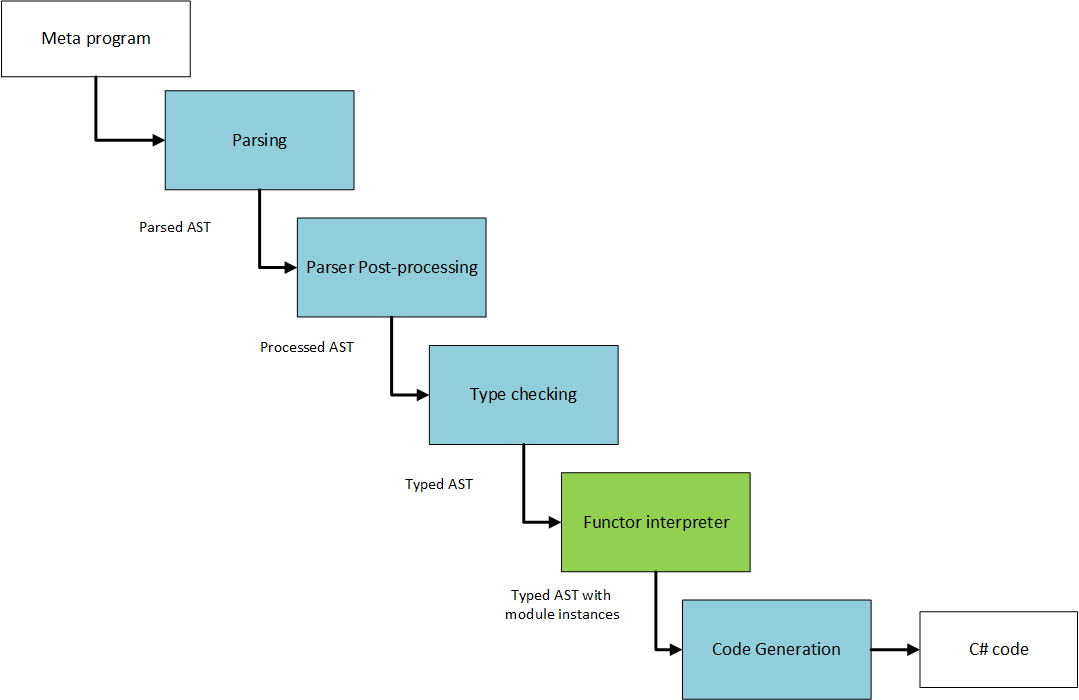
\includegraphics[width=\textwidth]{Figures/chapter_functors/compiler_architecture_functors}
	\caption{Compiler architecture with functor interpreter}
	\label{fig:ch_functors_compiler_architecture}
\end{figure}

\begin{figure}
	\centering
	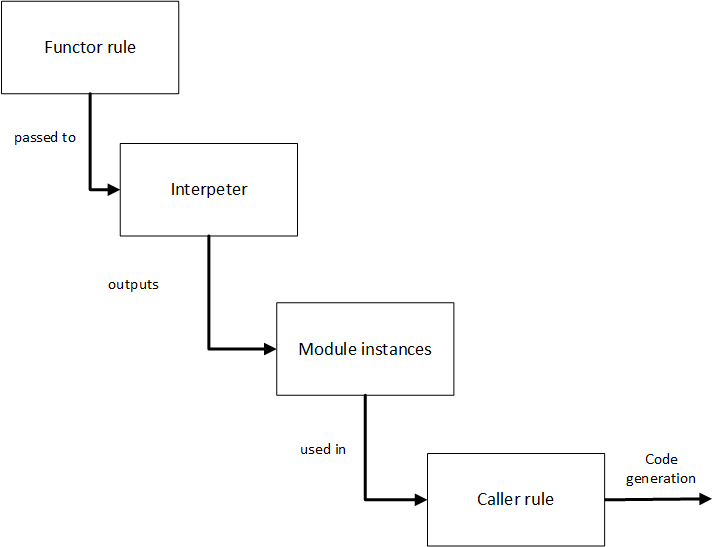
\includegraphics[width=\textwidth]{Figures/chapter_functors/functor_rule_processing}
	\caption{Functor processing}
	\label{fig:ch_functors_functor_processing}
\end{figure}

\section{Record implementation with modules}
\label{sec:ch_functors_record_implementation}
In Section \ref{subsec:ch_functors_inlining} we showed how Casanova entities can be expressed, at meta-language level, as a tuple of field names and values. We also showed that getters and setters always perform the same steps when looking up for the same field because the entity structure does not change at runtime. In this section we proceed to give an functor-based implementation of Casanova entities. We refer to this implementation as ``Record'', since a Casanova entity is simply a record from the point of view of the data representation. Moreover, since this solution works in general for any data structure that is isomorphic to a record. From now on we also use, as example, the physical body entity described in Section \ref{subsec:ch_functors_casanova_example}.

A module for records simply contains a functor that returns the type of the record. This functor, in general, can return any type since the type of the record can be ``customized'' and depends on the specific definition given by the programmer (thus it cannot be known beforehand). For this reason we use \textit{kind} as return type for this functor. The functor itself is parameterless since nothing is required to generate the type of a record.

\begin{lstlisting}
Module "Record" : Record {
  Functor "RecordType" : * }
\end{lstlisting}

The data representation of the record will be a tuple as shown in Section \ref{subsec:ch_functors_inlining}. For this purpose, we need two functors that are able to represent the type of a record in a recursive way with one being the type of an empty record (a record with no fields) and another a record field followed by the rest of the record representation. The functor for the empty record simply returns the type of the record module, while the functor to represent a record field takes as input a \texttt{string}, representing the name of the field, \textit{kind} because a record field can have any type, and a \texttt{Record} which represents all the other fields coming after the current one. 

\begin{lstlisting}
Functor "EmptyRecord" : Record
Functor "RecordField" => string => * => Record : Record
\end{lstlisting}

After declaring the functors necessary to build a record, we proceed to define their implementation in the form of rules. The functor for an empty record simply generates a module containing a function \texttt{cons}, that is the constructor for the record, that simply returns unit (because an empty record does not contain any field). Consistently, the functor \texttt{RecordType} implemented by the module will simply return \texttt{unit} as type. Note that a module instantiation must implement \textbf{at least} all the declarations of the module (like for an interface), but can add other declarations and implementations that are not shared by all the module instantiations. For example \texttt{cons} for an empty record is different than the one for a non-empty one.

\begin{lstlisting}
-------------------
EmptyRecord => Record {

  Func "cons" : unit
  
  ------------------
  RecordType => unit
  
  ------------------
  cons -> ()

}
\end{lstlisting}

A record field must be constructed through a functor that takes the field name, the type of the field, and the type of the rest of the record. This functor will construct the type of a record as a \texttt{Tuple}, where the first element is the type of the current field and the second the type of the rest of the record. The constructor of the record field will be a function that takes as input an argument of the type of the current field, a tuple representing the remaining part of the record and returns a tuple combining the current field and the rest of the record.

\begin{lstlisting}
------------------
RecordField name type r = Record {
  Func "cons" -> type -> r.RecordType : RecordType

  ---------------------------------------
  RecordType => Tuple[type,r.RecordType]

  -------------------
  cons x xs -> (x,xs)}
\end{lstlisting}

Consider now the physical body representation given above. We show how to use the functors we have just defined to build an instance of a physical body. First of all we defined a functor \texttt{PhysicalBodyType} that returns a \texttt{Record}.

\begin{lstlisting}
Functor "PhysicalBodyType" : Record
\end{lstlisting}

The final representation of the type that should be returned by\\ \texttt{PhysicalBodyType} is \texttt{Tuple[Vector2,Tuple[Vector2,unit]]} because the field\\ \texttt{Position} and \texttt{Velocity} have type \texttt{Vector2}. Note that \texttt{Vector2} can be trivially implemented in Metacasanova as a tuple containing two floating point values. Here we use this type assuming that has already been defined above. The same applies to \texttt{unit}, which can be defined as a meta-data with no arguments.

The rule to evaluate \texttt{PhysicalBodyType} will call in its premises\\ \texttt{EmptyRecord} and \texttt{RecordField} to generate the type of the tuple appropriately:

\begin{lstlisting}
EmptyRecord => empty
RecordField "Velocity" Vector2 empty => velocity
RecordField "Position" Vector2 velocity => body
----------------------------
PhysicalBodyType => body
\end{lstlisting}

Let us now analyse in detail what the premises generate: the first premise will generate an instance of \texttt{EmptyRecord} and bind it to the variable \texttt{empty}. The instance of this module is parameterless and thus will always be the same every time the functor is invoked. The second premise will instantiate \texttt{RecordField} by using the string \texttt{"Velocity"} as field name, \texttt{Vector2} as field type, and \texttt{empty} as argument for the remaining part of the record (there is no other field after \texttt{Velocity} in the physical body). The instantiation of \texttt{RecordField} produces a rule for the functor \texttt{RecordType}. According to the definition above this functor generates \texttt{Tuple[type,r.RecordType]}. By replacing the argument values provided in the premise, we have 

\begin{lstlisting}
type := Vector2
r := empty := EmptyRecord
\end{lstlisting}

\noindent
Thus \texttt{r.RecordType} uses the functor \texttt{RecordType} in the instance of\\ \texttt{EmptyRecord} which returns the type \texttt{unit} (the call can be seen as\\ \texttt{empty.RecordType}). Thus \texttt{r.RecordType} can be replaced with \texttt{unit}, thus leading to \texttt{Tuple[Vector2, unit]}. Thus the rule for the functor \texttt{RecordType} generated in the module returned by the second premise will be:

\begin{lstlisting}
-----------------------
RecordType => Tuple[Vector2,unit]
\end{lstlisting}

By replacing the argument variables with the values provided in the second premises we can also get the declaration and rule for \texttt{cons}. By replacing again \texttt{type} and \texttt{r.RecordType} as done before, we have that the declaration for \texttt{cons} in the current instance of the module becomes:

\begin{lstlisting}
Func "cons" -> Vector2 -> unit: Tuple[Vector2,unit]
\end{lstlisting}

\noindent
while the corresponding rule will be generated as

\begin{lstlisting}
--------------------
cons x xs -> (x,xs)
\end{lstlisting}

\noindent
The complete module instance will then look like:

\begin{lstlisting}
velocity := Record {
  Func "cons" -> Vector2 -> unit: Tuple[Vector2,unit]
  
  -----------------------
  RecordType => Tuple[Vector2,unit]
  
  --------------------
  cons x xs -> (x,xs)
}
\end{lstlisting}

The third premise calls \texttt{RecordField} with 

\begin{lstlisting}
name := "Position"
type := Vector2
r := velocity
\end{lstlisting}

\noindent
Now in the definition of the \texttt{RecordField} module again the functor\\ \texttt{RecordType} returns \texttt{Tuple[type,r.RecordType]}. Now \texttt{r.RecordType} can be rewritten as \texttt{velocity.RecordType} that returns (see the instantiation of \texttt{velocity} above) \texttt{Tuple[Vector2,unit]}. Thus \texttt{RecordType} for the field \texttt{Position} will be instantiated as

\begin{lstlisting}
-----------------------
RecordType => Tuple[Vector2,Tuple[Vector2,unit]]
\end{lstlisting}

\noindent
Analogously the declaration of \texttt{cons} will be instantiated as

\begin{lstlisting}
Func "cons" -> Vector2 -> Tuple[Vector2,unit]: Tuple[Vector2,Tuple[Vector2,unit]]
\end{lstlisting}

\noindent
while its rule is the same of the second premise. The full module instance will then be

\begin{lstlisting}
body := Record {
  Func "cons" -> Vector2 -> Tuple[Vector2,unit]: Tuple[Vector2,Tuple[Vector2,unit]]
  
  -----------------------
  RecordType => Tuple[Vector2,Tuple[Vector2,unit]
  
  --------------------
  cons x xs -> (x,xs)
}
\end{lstlisting}

\noindent
which is returned by the functor \texttt{PhysicalBodyType}. In order to build an instance of the physical body, we define a function that returns a value of type \texttt{PhysicalBodyType}. which in turn is simply \texttt{Tuple[Vector2,\\Tuple[Vector2,unit]}):

\begin{lstlisting}
Func "PhysicalBody" : PhysicalBodyType.RecordType

-----------------------
PhysicalBody -> PhysicalBodyType.cons((10.0,10.0),((10.0,0.0),()))
\end{lstlisting}

\noindent
The rule creates a physical body in position $(10,10)$ moving at velocity $(10,0)$.\\

One of the main arguments in favour of using functors was that they should allow to embed the type system of the embedded language in the meta-type system of Metacasanova. This means that, at compile time, the meta-compiler should be able to detect a physical body that is constructed in the wrong way. Let us then assume that we define another function to build a physical body where the programmer uses a scalar for the velocity instead of a vector:

\begin{lstlisting}
Func "WrongPhysicalBody" : PhysicalBodyType.RecordType

-------------------------------------
WrongPhysicalBody ->  PhysicalBodyType.cons((10.0,10.0),(10.0,()))
\end{lstlisting}

\noindent
What happens is that \texttt{PhysicalBodyType.RecordType} is equal to\\ \texttt{Tuple[Vector2,Tuple[Vector2,unit]]}. At this point the type checker of Metacasanova will successfully match the first element of the tuple returned by the rule, which is correctly provided as a value of type \texttt{Vector2}, but will fail to check the second, which is \texttt{double} where it expects a \texttt{Vector2}. This check happens statically, rather than dynamically at runtime as was the case with the implementation based on dictionaries in Section \ref{subsec:ch_mcnv_languages_casanova_semantics}.

\section{Getting Values from Record Fields}
\label{sec:ch_functors_record_getter}
Getting a value from a record field requires defining a module \texttt{Getter} containing a functor \texttt{GetField} that returns the type of the field that we need to get. This type will be used as the return type of the function \texttt{get} that is able to get that specific field. This function is also contained in this module and takes as argument the record from which we are getting the value and returns, as said above, the value of the field. The module \texttt{Getter} is built using the name of the field that is able to read and the record to read from.

\begin{lstlisting}
Module "Getter" => (name : string) => (r : Record) : Getter { ... }
\end{lstlisting}

The functor \texttt{GetType} returns kind because in general the type of the field of a record is arbitrary. The function \texttt{get} uses in its declaration the functor \texttt{RecordType} to determine the type of the record to use and \texttt{GetType} to determine the type of the field to read. The complete module will look like

\begin{lstlisting}
Module "Getter" => (name : string) => (r : Record) : Getter {
  Functor "GetType" : *
  Func "get" -> (r.RecordType) : GetType
}
\end{lstlisting}

\noindent
The getter has two implementations of the rule that instantiates the \texttt{Getter} module: one is used when the current field in the module tuple is the one we are trying to read, and the other that is able to build the correct getter if the field is in the remaining part of the record. The first happens when the name of the current field is the same as the field name provided as argument of the functor \texttt{GetField}. In this case we have the following rule for the functor:

\begin{lstlisting}
Functor "GetField" => string => Record : Getter
\end{lstlisting}

\begin{lstlisting}[caption = Getting a field (case 1),label = lst:ch_functors_getter1]
name = fieldName
thisRecord := RecordField name type r
--------------------------------------
GetField fieldName (RecordField name type r) => Getter fieldName thisRecord {
  
  ---------------
  GetType => type
  
  ---------------
  get (x,xs) -> x
}
\end{lstlisting}

\noindent
The functor \texttt{GetType} simply returns the type of the current record field, because it is the correct field to read, and \texttt{get} returns the first element of the record tuple, which represents the value stored in the field itself.

When the field we are trying to read is not the one we are currently examining in the record tuple, we must build a getter functor that is able to recursively get the field from the remaining part of the record. At this purpose, we have to extend the \texttt{Getter} with an additional functor \texttt{GetAnotherField} that returns a module instance capable of reading the value from the correct field in the remaining part of the record and its type. The implementation of the rule for this case is the following:

\begin{lstlisting}[caption = Getting a field (case 2),label = lst:ch_functors_getter2]
name <> fieldName
thisRecord := RecordField name type r
-------------------------------------
GetField fieldName (RecordField name type r) => Getter fieldName type thisRecord {
		Functor "GetAnotherField" : Getter
		
		GetField fieldName r => otherGetter
		------------------------------
		GetAnotherField => otherGetter
		
		GetAnotherField => g
		---------------------
		GetType => g.GetType
		
		GetAnotherField => getter
		getter.get xs -> v
		------------------
		get (x,xs) -> v
  }
}
\end{lstlisting}

\noindent
The rule for the functor \texttt{GetAnotherField} simply calls recursively the rule for \texttt{GetField} with the remaining part of the record. If the next field is the correct one then this time we will use the rule in Listing \ref{lst:ch_functors_getter1}, otherwise the rule in Listing \ref{lst:ch_functors_getter2} will be re-applied until the correct field is reached. The functor \texttt{GetType} simply calls \texttt{GetAnotherField} to obtain the module instance necessary to get the field from the rest of the record, and then calls the functor \texttt{GetType} from that instance. Finally, the function \texttt{get} will again use \texttt{GetAnotherField} and then call the \texttt{get} function from the getter returned by \texttt{GetAnotherField} with the remaining part of the record tuple. This function call will return the desired value that will be used also as result of the current \texttt{get}.

Let us now consider again the physical body implemented with functors in Section \ref{sec:ch_functors_record_implementation} and let us assume that we want to get the value of the field \texttt{Position}. We define a function \texttt{getPos} that takes as input a physical body and returns \texttt{Vector2}. This function will use \texttt{GetField} in its premises to generate the getter for \texttt{Position} and will then call the \texttt{get} function from the generated module instance.

\begin{lstlisting}[caption = Getter for the Position field, label = lst:ch_functors_position_getter]
Func "getPos" : Vector2

GetField "Position" PhysicalBodyType => getter
PhysicalBody -> body
getter.get body -> p
-----------------
getPos -> p
\end{lstlisting}

\noindent
Note that in the code above we are using the functor \texttt{PhysicalBodyType} and the function \texttt{PhysicalBody} defined in Section \ref{sec:ch_functors_record_implementation}. Now let us analyse step-by-step what happens when we call \texttt{getPos}. The first premise will call the functor \texttt{GetField} with 

\begin{lstlisting}
fieldName := "Position"
r := PhysicalBodyType := RecordField "Position" Vector2 (RecordField "Velocity" Vector2 EmptyRecord)
\end{lstlisting}

\noindent
At this point the rule for \texttt{GetField} will deconstruct \texttt{RecordField} in its conclusion by means of pattern matching and set 

\begin{lstlisting}
name := "Position"
type := Vector2
r := RecordField "Velocity" Vector2 EmptyRecord
\end{lstlisting}
 
\noindent
Since \texttt{name} = \texttt{fieldName} we fall in the case in Listing \ref{lst:ch_functors_getter1}. Thus we instantiate the module \texttt{Getter} by setting the construction arguments to 

\begin{lstlisting}
name := "Position"
r := RecordField "Position" Vector2 (RecordField "Velocity" Vector2 EmptyRecord)
\end{lstlisting}

\noindent
In this module instance the functor \texttt{GetType} returns \texttt{type :=  Vector2} and \texttt{get} returns the first element of the record tuple. At this point, the third premise will call \texttt{get} from this module instance by passing the record tuple\\ \texttt{((10.0,10.0),((10.0,0.0),()))}, which in turn returns correctly \texttt{(10.0,10.0)}.

Now let us assume that we want to retrieve the value of "Velocity" instead. We define an analogous function \texttt{getVel} as follows

\begin{lstlisting}
Func "getVel" : Vector2

GetField "Velocity" PhysicalBodyType => getter
PhysicalBody -> body
getter.get body -> v
-----------------
getVel -> v
\end{lstlisting}

\noindent
This time the functor \texttt{GetField} is called with

\begin{lstlisting}
fieldName := "Velocity"
r := PhysicalBodyType := RecordField "Position" Vector2 (RecordField "Velocity" Vector2 EmptyRecord)
\end{lstlisting}

\noindent
thus the rule in case 2 is triggered. This rule will generate an instance of \texttt{Getter}

\begin{lstlisting}
fieldName := "Velocity"
type := Vector2
r := RecordField "Velocity" Vector2 EmptyRecord
\end{lstlisting}

\noindent
This rule will generate a module containing the auxiliary functor \texttt{GetAnotherField} that is capable to retrieve the correct field in the remaining part of the record. The rule that processes \texttt{GetAnotherField} will call, in its premise, \texttt{GetField} with

\begin{lstlisting}
fieldName := "Velocity"
r := RecordField "Velocity" Vector2 EmptyRecord
\end{lstlisting}

Since now the name of the field of the getter coincides with the name of the field in \texttt{RecordField}, this premise will now trigger the rule in Listing \ref{lst:ch_functors_getter2} that in turn generates an instance of \texttt{GetField} containing the following:

\begin{lstlisting}[caption = Getter for Velocity generated by \texttt{GetAnotherField}, label = lst:ch_functors_velocity_getter2]
Func "get" -> Tuple[Vector2,unit] : Vector2

-------------------
GetType => Vector2


----------------
get (x,xs) -> x
\end{lstlisting}

\noindent
This module instance will be the one returned by the rule of \texttt{GetAnotherField}. The rule of the functor \texttt{GetType} for \texttt{Velocity} will use \texttt{GetAnotherField} to retrieve the correct field type using the module instance generated in Listing \ref{lst:ch_functors_velocity_getter2} and return it (which is \texttt{Vector2}). The rule for the function \texttt{get} will use \texttt{GetAnotherField} to call the the \texttt{get} function from Listing \ref{lst:ch_functors_velocity_getter2} passing the second element of the record tuple as argument and returns the result of this function call.

Note that the module instantiation will be again performed at compile time, thus the only operations performed at runtime are the calls to the \texttt{get} functions contained in the module instantiations.

\section{Setting Values of Record Fields}
\label{sec:ch_functors_record_setter}
The setter module is analogous to the getter, except that this time the module must generate a function that, in addition to the record, takes as input the value to write in the field. This function returns a modified copy of the record tuple where the value associated to the field has been changed. For this purpose we need a module containing a functor \texttt{SetType} that returns the type of the field to set. This functor will be used to build the declaration of a function \texttt{set} that is able to set the specified field.

\begin{lstlisting}
Module "Setter" => (name : string) => (r : Record) : Setter {
	Functor "SetType" : *
	Func "set" -> r.RecordType -> SetType : r.RecordType
}
\end{lstlisting}

\noindent
The declaration of the function \texttt{set} uses \texttt{r.RecordType} to define the type of the record argument, \texttt{SetType} to define the type of the field to set, necessary for the argument containing the value to set, and returns \texttt{r.RecordType}, which is the modified version of the record.

Analogously to the getter, we need a functor that instantiates \texttt{Setter} and has two different implementations of the instantiation rule: one where the field of the current element of the record tuple coincides with the one we want to set, and the other where the field is different and that is able to build a setter for the remaining part of the record tuple.

\begin{lstlisting}
Functor "SetField" => string => Record : Setter
\end{lstlisting}

The first case is implemented as follows:

\begin{lstlisting}[caption = Setting a field (case 1), label = lst:ch_functors_setter1]
name = fieldName
thisRecord := RecordField name type r
------------------------------
SetField fieldName (RecordField name type r) => Setter fieldName thisRecord {

  ----------------
  SetType => type
  
  ----------------------
  set (x,xs) v -> (v,xs)
}
\end{lstlisting}

\noindent
The function \texttt{SetType} simply returns the type of the field in the current \texttt{RecordField}, while the rule for \texttt{set} replaces the first value in the record tuple with the new value. The second rule is implemented as follows

\begin{lstlisting}[caption = Setting a field (case 2), label = lst:ch_functors_setter2]
name <> fieldName
thisRecord := RecordField name type r
-------------------------------------
SetField fieldName (RecordField name type r) => Setter fieldName thisRecord {
  Functor "SetAnotherField" : Setter
  
  SetField fieldName r => setter
  -------------------------------
  SetAnotherField => setter
  
  SetAnotherField => s
  -------------------------
  SetType => s.SetType
  
  SetAnotherField => setter
  setter.set xs v -> xs'
  ----------------------
  set (x,xs) v -> (x,xs')
}
\end{lstlisting}

\noindent
The functor \texttt{SetAnotherField} is an auxiliary functor that recursively calls\\ \texttt{SetField} with the remaining part of the record. Eventually \texttt{SetField} will trigger the rule in Listing \ref{lst:ch_functors_setter1} when the correct field is encountered. This auxiliary functor is then used in \texttt{SetType} to retrieve the correct type of the record field and in the function \texttt{set} to call the correct \texttt{set} function for the field. The \texttt{set} function in the setter generated by \texttt{SetAnotherField} returns a modified version of the record that is replaced in the tuple.

Let us now consider again the physical body and assume that we want to define a setter for \texttt{Position}. Again we define a function \texttt{setPos} for the field:

\begin{lstlisting}
Func "setPos" -> Vector2 : PhysicalBodyType

SetField "Position" PhysicalBodyType => setter
PhysicalBody -> body
setter.set body -> body'
-----------------------
setPos v -> body'
\end{lstlisting}

\noindent
Again we are using the functor \texttt{PhysicalBodyType} and the function\\ \texttt{PhysicalBody} defined in Section \ref{sec:ch_functors_record_implementation}. The first premise of this rule will call \texttt{SetField} with

\begin{lstlisting}
fieldName := "Position"
name := "Position"
type := Vector2
r := RecordField "Velocity" Vector2 EmptyRecord
\end{lstlisting}

\noindent
which, in turn, instantiates \texttt{Setter} with 

\begin{lstlisting}
name := "Position"
r := RecordField "Position" Vector2 (RecordField "Velocity" Vector2 EmptyRecord)
\end{lstlisting}

\noindent
In this module instance \texttt{r.RecordType} will be\\ \texttt{Tuple[Vector2,Tuple[Vector2,unit]]} and \texttt{SetType} returns \texttt{Vector2}. The whole instance will look like

\begin{lstlisting}
Func "set" -> Tuple[Vector2,Tuple[Vector2,unit]] -> Vector2 : Tuple[Vector2,Tupe[Vector2,unit]]

------------------
SetType => Vector2


----------------------
set (x,xs) v -> (v,xs)
\end{lstlisting}

\noindent
Now let us assume that we want to build a setter for \texttt{Velocity}. We have to define a function \texttt{setVel} as follows

\begin{lstlisting}
Func "setVel" -> Vector2 : PhysicalBodyType

SetField "Velocity" PhysicalBodyType => setter
PhysicalBody -> body
setter.set v -> body'
-------------------------
setVel v -> body'
\end{lstlisting}

\noindent
The first premise of this rule will now invoke \texttt{SetField} with

\begin{lstlisting}
fieldName := "Velocity"
name := "Position"
type := Vector2
r := RecordField "Velocity" Vector2 EmptyRecord
\end{lstlisting}

\noindent
which will trigger the rule in Listing \ref{lst:ch_functors_setter2} instead. This will create an instance of \texttt{Setter} containing  the auxiliary functor \texttt{SetAnotherField}. The rule for this functor will call in turn \texttt{SetField} with

\begin{lstlisting}
fieldName := "Velocity"
name := "Velocity"
type := Vector2
r := EmptyRecord
\end{lstlisting}

\noindent
that will generate a different instance of \texttt{Setter}, this time using the rule in Listing \ref{lst:ch_functors_setter1}. The auxiliary setter will contain a functor \texttt{SetType} returning \texttt{Vector2} and a function \texttt{set} that inserts the value for \texttt{Velocity} in the record tuple. The \texttt{set} in the auxiliary setter will be used in the setter of \texttt{Velocity} to obtain the modified copy of the record containing the new value. Again all the modules are generated at compile time, thus the only operations performed at runtime are the calls to the \texttt{set} functions of the field setter and eventual auxiliary modules.

\section{Handling errors in getters and setters}
\label{sec:ch_functors_error_handling}
In Section \ref{sec:ch_functors_record_getter} and \ref{sec:ch_functors_record_setter} we explained how to use functors to implement getters and setters for the fields of a record. The explanation however did not take into account possible mistakes that could be committed during the definition of setters and getters for a specific record.

A possible mistake that could arise in the process of defining getters and setters would be to provide an incompatible type for the \texttt{get} function of a field. For instance, let us assume that we define \texttt{getPos} as

\begin{lstlisting}
Func "wrongGetPos" : double

GetField "Position" PhysicalBodyType => getter
PhysicalBody -> body
getter.get body -> v
-----------------
wrongGetPos -> v
\end{lstlisting}

\noindent
As explained above the getter module will contain a function \texttt{get} that returns a \texttt{Vector2}, because that is the type of the field \texttt{Position}. In the process of building the module, this type is automatically retrieved from the definition of \texttt{PhysicalBodyType}. At this point the meta-compiler would report an error message because this wrong definition of \texttt{getPos} returns \texttt{double} but \texttt{get} returns a \texttt{Vector2}. Note that, as previously explained in Section \ref{sec:ch_functors_record_implementation}, this is possible because functors are able to embed the type system of the embedded language into the Metacasanova type system.


Another possible mistake is accessing a field that is not defined for the record. For instance, let us assume that someone tries to build a getter for a field that does not exist in physical body, namely a field \texttt{Acceleration}. As usual we would define a function for the getter such as

\begin{lstlisting}
Func "getAcc" : Vector2

GetField "Acceleration" PhysicalBodyType => getter
PhysicalBody -> body
getter.get body -> v
---------------
getAcc -> v
\end{lstlisting}

\noindent
The first premise of this rule will call the functor \texttt{GetField} with

\begin{lstlisting}
fieldName := "Acceleration"
name := "Position"
type := Vector2
r := RecordField "Velocity" Vector2 EmptyRecord
\end{lstlisting}

\noindent
As seen above, this rule will generate an auxiliary module by recursively call \texttt{GetField} with

\begin{lstlisting}
fieldName := "Acceleration"
name := "Velocity"
type := Vector2
r : = EmptyRecord
\end{lstlisting}

\noindent
but at this point, since again \texttt{fieldName} $\neq$ \texttt{name} we will recursively call \texttt{GetField}. At this point we will fail to run a suitable rule for the functor, since the only two versions we have so far are able to process \texttt{RecordField} and not \texttt{EmptyRecord}, thus the pattern matching in the conclusion would fail. The meta-compiler will in any case fail to generate code, since the functor evaluation will fail and thus the whole code generation, but this approach is not ``clean'', since the meta-compiler will report a generic error regarding the rule execution failure. An alternative to this, is to include a case for the rule that processes \texttt{EmptyRecord}. A getter for an \texttt{EmptyRecord} returns \texttt{()} and \texttt{GetType} returns the type \texttt{unit}. This rule can be implemented as follows:

\begin{lstlisting}

fieldName <> name
thisRecord := RecordField name type EmptyRecord
-------------------------------
GetField fieldName (RecordField name type EmptyRecord) => Getter fieldName thisRecord {
	
  ----------------
  GetType => unit
  
  ----------------
  get (x,xs) -> ()
}
\end{lstlisting}

In this way the first premise of the rule of \texttt{getAcc} would generate a getter that takes a physical body and returns \texttt{unit}. When the rule calls this getter and returns \texttt{unit}, this will be incompatible with the return type of \texttt{getAcc} that should be a \texttt{Vector2}. The same can be done for \texttt{setAcc}, that is we extend the rule for \texttt{SetField} with an additional case:

\begin{lstlisting}
fieldName <> name
thisRecord := RecordField name type EmptyRecord
--------------------------
SetField fieldName (RecordField name type EmptyRecord) => Setter fieldName thisRecord {
	
	----------------
	SetType => unit
	
	----------------------
	set (x,xs) v -> (x,xs)
}
\end{lstlisting}

\noindent
In this way, when invoking \texttt{set} in the premise \texttt{setAcc} the compiler will signal a type error because at some point it will try to use the \texttt{set} for the \texttt{EmptyRecord} with \texttt{Vector2}. Another alternative, which goes beyond the scope of this chapter, would be to allow rules in meta-casanova to output custom compilation errors. In this way we could write the very same rule case done above but this time we would return a compilation error message reporting that the field does not exist.

\section{Evaluation}
\label{sec:ch_functors_evaluation}
In the previous sections we presented an extension to the meta-language of Metacasanova that allows to embed the type system of an embedded language, whose definition is implemented in Metacasanova, in the meta-type system of Metacasanova. We claimed that this would improve the runtime performance of a program written in the embedded language because we could get rid of all the dynamic checks and accesses to meta-data structures used to implement data structures in the embedded language, such as records. In this section we present the experimental evaluation that should produce the evidence to back up this claim. We proceed to describe the experimental set-up and then we comment the results.

\subsection{Experimental Set-up}
In this experiment we use the implementation of records with functors described in this chapter and we compare its runtime performance with its dynamic counter part, i.e. the implementation that uses dictionaries, that was used to implement the Casanova memory model in Section \ref{subsec:ch_mcnv_languages_casanova_semantics}. The sample measures the run-time of both the functor implementation and the implementation with dynamic tables. We run the test by varying both the number of record instances and the number of fields per record. The test is run with a sample of 10000, 100000, and 1000000 record instances and with a number of fields from 1 to 10. We neglect to consider different field types, as the performance of look-up operations is not affected by the type of the fields themselves.

\subsection{Results}

In Table \ref{tab:ch_functors_results}, we can see that the optimization using Functors leads to a performance increase on average of about 11 times, with peaks of 30 times. The gain increases with the number of fields, thus the implementation with functors is particularly effective for records with high number of fields. This is due to the fact that the runtime complexity of a dynamic table depends on the number of entries stored in it (which would be the fields in our case) and thus, when the fields are few, this number is very close to the complexity of the functorial implementation, which is constant. When the number of fields increases, the performance of the functorial implementation remains the same while the dynamic table one worsens visibly. The constant complexity of the functorial implementation is due to the fact that the meta-compiler builds the functions of a getter or setter module instance, used to look up a specific field or set its value, at compile time by generating the appropriate module instances with the functors. The \texttt{get} and \texttt{set} functions described above can either immediately get or set the value of the field and return the result of this operation, or call the getter or setter of an auxiliary module instance that is able to read or write the appropriate field. The only overhead is the overhead of chaining calls to Metacasanova functions, thus the overhead of creating and executing the code that implements the rule behaviour described in Section \ref{sec:ch_metacasanova_code_generation}.

Figure \ref{fig:ch_functors_chart} shows a chart of the overall performance of the two techniques (the data points are taken from Table \ref{tab:ch_functors_results}). The horizontal axis contains the number of fields per record, while the vertical axis contains the number of records that are being updated. We can see that the performance of the dynamic table degrades considerably when increasing the number of fields, and that the higher the number of records is, the steeper the curve is. On the other hand, the performance of the implementation with functors is almost constant, regardless of the number of fields or records that are being updated. Moreover, note that the performance of the dynamic table is improved by the fact that we are using a dictionary implemented in .NET. If the symbol table were represented as a meta-data structure in the language, the performance would be even worse, since it would have to be encoded as a list of pairs with the field name and its value, and its manipulation would be affected by the evaluation rules that should implement this behaviour. Furthermore, the dynamic lookup should be done also to ensure that the types of the record fields are used consistently (which is not accounted for here, for example to prevent that a record is constructed with incompatible values for its fields), while this check is done at compile time with functors, thus drastically improving the performance.

\subsubsection{Dynamic Table implementation Choice}
After both these considerations and those presented in Chapter \ref{sec:ch_mcnv_languages_evaluation} a legitimate doubt could be uttered about the choice of the implementation of the dynamic tables. We mentioned multiple times that we chose to use a tree-based implementation of the dictionary, but a valid objection could be that one could use a HashTable whose complexity is $O(1)$. This assumption cannot be applied to this case for the following reasons:

\begin{itemize}
\item The hash table access operations have a complexity of $O(1)$ when the number of entries stored in it is very big. Indeed the definition of big-oh states that $f(n) = O(g(n))$ if
\begin{align*}
\exists c \in \mathbb{R}: \lim_{n \to \infty}\dfrac{f(n)}{g(n)} = c
\end{align*}
\noindent
thus it makes sense to talk in term of complexity only if the size of the table is very large. It is very unlikely that a record will contain a large number of fields. In this scenario, the performance of a hash table decays because the running time is affected by the computation of the hash function for every access and the resize of the table performed to decrease the load factor in order to minimize the number of collisions \cite{cormen2001introduction}. In the case of records, where the amount of fields and thus of entries in the table is limited, the performance of the tree implementation and the hash table are on the same order of magnitude.
\item  Metacasanova is a referentially transparent language, as all data structures are immutable. Referential transparency is a desirable property to have because it helps in the verification of the correctness of programs \cite{linger1988case, trammell1996incremental} and prevents side-effects. Hash tables have high performance only when mutability is allowed, but implementing an immutable hash table requires to recreate the whole table inserting all the entries again by re-hashing them. This does not happen in trees, where we do not need to recreate the whole tree but only the sub-tree that is affected by the manipulation of the data structure.
\end{itemize}

\begin{table}
	\centering
	\begin{tabular}{|c|c|c|c|}
		\hline
		\textbf{FIELDS}& \textbf{Functors (ms)}&\textbf{Dynamic Table (ms)} & \textbf{Gain}\\ \hline
		1&	1.00E-05&	5.00E-06&	0.50\\ \hline
		2&	9.00E-06&	1.30E-05&	1.44\\ \hline
		3&	9.00E-06&	2.70E-05&	3.00\\ \hline
		4&	9.00E-06&	4.50E-05&	5.00\\ \hline
		5&	9.00E-06&	7.00E-05&	7.78\\ \hline
		6&	9.00E-06&	9.90E-05&	11.00\\ \hline
		7&	9.00E-06&	1.33E-04&	14.78\\ \hline
		8&	9.00E-06&	1.75E-04&	19.44\\ \hline
		9&	9.00E-06&	2.20E-04&	24.44\\ \hline
		10&	9.00E-06&	2.70E-04&	30.00\\ \hline
		\multicolumn{2}{c|}{} & \textbf{Average gain} & 11.74\\ \cline{3-4}			
	\end{tabular}
	
	\vspace{0.15cm}
	\begin{tabular}{|c|c|c|c|}
		\hline
		\textbf{FIELDS}& \textbf{Functors (ms)}&\textbf{Dynamic Table (ms)} & \textbf{Gain}\\ \hline
		1&	9.60E-05&	6.30E-05&	0.66\\ \hline
		2&	9.40E-05&	1.59E-04&	1.69\\ \hline
		3&	9.50E-05&	3.04E-04&	3.20\\ \hline
		4&	9.60E-05&	5.03E-04&	5.24\\ \hline
		5&	9.60E-05&	7.52E-04&	7.83\\ \hline
		6&	9.60E-05&	1.05E-03&	10.95\\ \hline
		7&	9.70E-05&	1.41E-03&	14.57\\ \hline
		8&	9.80E-05&	1.82E-03&	18.59\\ \hline
		9&	9.90E-05&	2.29E-03&	23.17\\ \hline
		10&	1.00E-04&	2.81E-03&	28.05\\ \hline
		\multicolumn{2}{c|}{} & \textbf{Average gain} & 11.39\\ \cline{3-4}						
	\end{tabular}
	
	\vspace{0.15cm}
	\begin{tabular}{|c|c|c|c|}
		\hline
		\textbf{FIELDS}& \textbf{Functors (ms)}&\textbf{Dynamic Table (ms)} & \textbf{Gain}\\ \hline
		1&	9.47E-04&	7.29E-04&	0.77\\ \hline
		2&	9.51E-04&	1.78E-03&	1.87\\ \hline
		3&	9.50E-04&	3.33E-03&	3.51\\ \hline
		4&	9.60E-04&	5.43E-03&	5.66\\ \hline
		5&	9.65E-04&	8.03E-03&	8.32\\ \hline
		6&	9.71E-04&	1.11E-02&	11.44\\ \hline
		7&	9.75E-04&	1.47E-02&	15.12\\ \hline
		8&	9.82E-04&	1.89E-02&	19.28\\ \hline
		9&	9.92E-04&	2.37E-02&	23.86\\ \hline
		10&	1.00E-03&	2.87E-02&	28.62\\ \hline
		\multicolumn{2}{c|}{} & \textbf{Average gain} & 11.84\\ \cline{3-4}						
	\end{tabular}
 	\caption{Running time with the functor optimization and the dynamic table with 10000, 100000, and 1000000 records.}
	\label{tab:ch_functors_results}
\end{table}

\begin{figure}
	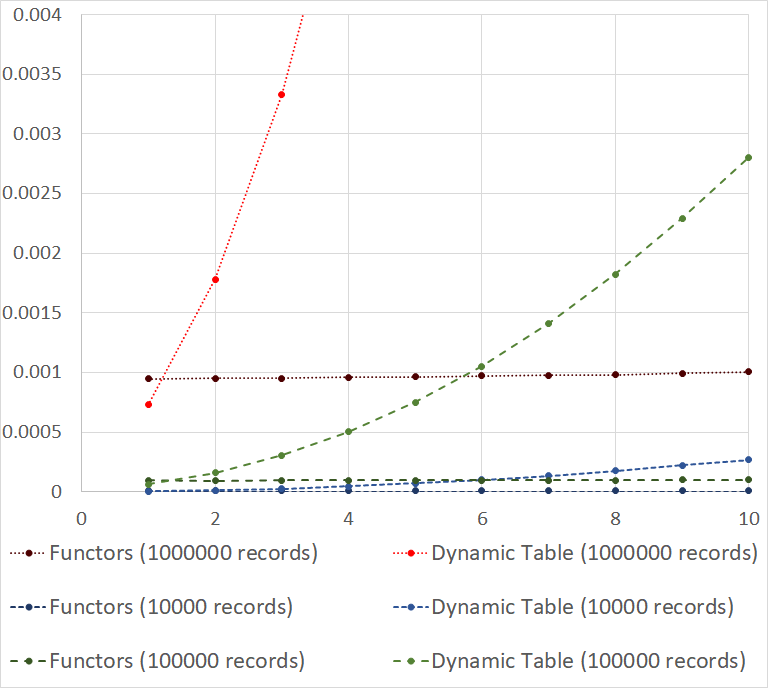
\includegraphics[width = \textwidth]{Figures/chapter_functors/functor_chart}
	\caption{Execution time of the different memory models}
	\label{fig:ch_functors_chart}
\end{figure}

\section{Summary}
In this chapter we addressed the problem described in Section \ref{sec:ch_mcnv_languages_evaluation} about the performance of the generated code and the forced dynamic behaviour of languages implemented in Metacasanova. We started by informally state that this issue was due to the fact that it was not possible to embed the type system of a language in the meta-type system of Metacasanova, and this caused all the dynamic lookups and accesses at runtime. This issue can be avoided by using a meta-language abstraction that allows both to define the type system of the embedded language in terms of the meta-type system of Metacasanova and to generate the code for the accesses to the data structures of the embedded language at compile time. For this purpose, we proposed a language extension that provides such abstraction in terms of modules and functors. We then proceeded to provide an example of their usage in the context of record getters and setters for their fields. We then measured the performance gain by comparing the implementation with functors with the one using dynamic tables that was employed for the Casanova language implementation shown in Section \ref{subsec:ch_mcnv_languages_casanova_semantics}. The results show that the performance of operations on records in the case of functors is up to 30 times faster than the dynamic table implementation. We have also shown that the performance of such operations in the case of functors is constant with respect to the number of fields to update, while the performance of the dynamic table drastically worsens when the number of fields in a record increases. In the next chapter we will show a further example of use of functors to re-implement Casanova semantics and extend the language with abstractions to express the networking behaviour for multiplayer games.


\section{Evaluation}
\label{sec:evaluation}
GrandeOmega has been tested extensively with students from Hogeschool Rotterdam, a university of applied science in the Netherlands. The classes were divided into two groups: in the first classes were given some programming assignments to be completed in the traditional way (without GrandeOmega), while in the second other classes were asked to solve the assignments both in the traditional way and in GrandeOmega. Table \ref{tab:performance_go} and Figure \ref{fig:bar_chart} contain data relative to the pass rate and average grades of the classes that were asked to used also GrandeOmega, with and without using it. Table \ref{tab:prediction} and Figure \ref{fig:prediction} contain data relative to the accuracy of the prediction on the student success performed by GrandeOmega. The total number of students who participated is 241.

The data shows that the use of GrandeOmega enhanced the pass rate of classes 1B and 1C, but not that of 1F, 1L, and 1A. This means that the students of 1B and 1C failed questions in the traditional way that they were able to solve in GrandeOmega. Nonetheless, we can see that it always enhanced the grades of all the classes by at least 4\%. Moreover, if we compare the average passing grade of these classes with those who never used GrandeOmega, we can see that we reach a difference of even 12\%.

GrandeOmega was revealed to be effective even in predicting the success of students with a total reliability of 77\%, based on the percentage of assignment completed correctly.

\begin{table}[!h]
	\begin{tabular}{|p{0.1\columnwidth}|p{0.1\columnwidth}|p{0.1\columnwidth}|p{0.1\columnwidth}|p{0.1\columnwidth}|p{0.1\columnwidth}|}
		\hline
		\textbf{Class} & Completions & Pass rate & Pass rate G.O. & Average grade & Average grade G.O. \\
		\hline
		INF1B & 71.8 & 3 & 14 & 84.7 & 97.2 \\
		\hline
		INF1F & 56.7 & 6 & 5 & 77.0 & 88.1 \\
		\hline
		INF1L & 48.1 & 2 & 2 & 75 & 83.8 \\
		\hline
		INF1A & 41.7 & 7 & 7 & 82.1 & 86.5 \\
		\hline
		INF1C & 35.6 & 5 & 7 & 82.5 & 93.3 \\
		\hline
	\end{tabular}
	\caption{Student performance before and after GrandeOmega}
	\label{tab:performance_go}
\end{table}

\begin{table}[!h]
	\begin{tabular}{|p{0.2\textwidth}|p{0.2\textwidth}|p{0.2\textwidth}|p{0.2\textwidth}|p{0.2\textwidth}|}
		\hline
		\textbf{Class} & \textbf{Correct prediction} & \textbf{False positive} & \textbf{False negative} & \textbf{Incorrect prediction} \\
		\hline
		INF1B & 16 & 8 & 2 & 10 \\
		\hline
		INF1F & 11 & 2 & 4 & 6 \\
		\hline
		INF1L & 18 & 3 & 1 & 4 \\
		\hline
		INF1A & 13 & 0 & 2 & 2 \\
		\hline
		INF1C & 15 & 1 & 1 & 2 \\
		\hline
	\end{tabular}
	\caption{Prediction of student performance}
	\label{tab:prediction}
\end{table}

\begin{table}[!h]
	\begin{tabular}{|p{0.25\textwidth}|p{0.25\textwidth}|p{0.25\textwidth}|p{0.25\textwidth}|}
		\hline
		\textbf{Class} & \textbf{Average grade} & \textbf{Passed students} & \textbf{Avarage passing grade} \\
		\hline
		INF1H & 41.4 & 3 & 83.3 \\
		\hline
		INF1E & 30.6 & 1 & 75 \\
		\hline
		INF1J & 23.3 & 0 & N.A. \\
		\hline
		INF1G & 41.4 & 7 & 80.3 \\
		\hline
	\end{tabular}
	\caption{Results of classes without GrandeOmega}
	\label{tab:performance_no_go}
\end{table}

\begin{figure}[!h]
	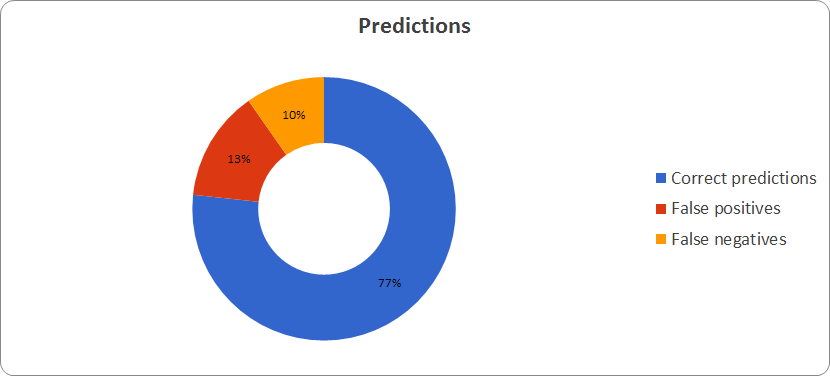
\includegraphics[width = \columnwidth]{Figures/prediction}
	\caption{Predition accuracy of GrandeOmega}
	\label{fig:prediction}
\end{figure}

\begin{figure}[!h]
	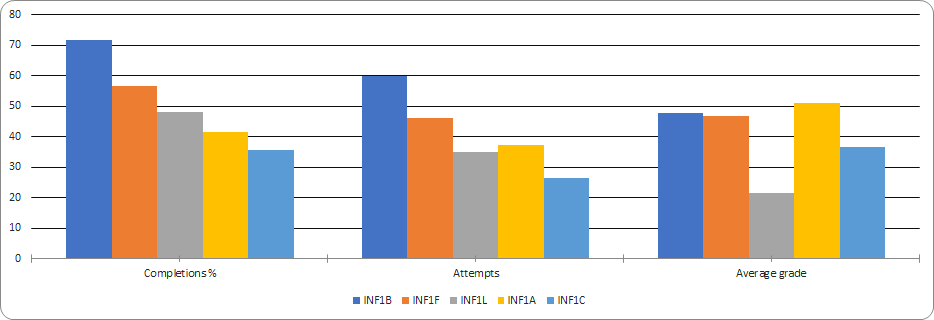
\includegraphics[width = \columnwidth]{Figures/bar_chart}
	\caption{Student performance with and without G.O.}
	\label{fig:bar_chart}
\end{figure}

\section{Conclusion}
\label{sec:conclusion}
In this work we addressed the problem of teaching and learning how to program and we proposed the use of a didactic model called GrandeOmega. The web implementation of GrandeOmega was tested on a subset of students from Hogeschool Rotterdam with promising results: the use of the didactic model managed, in some cases, to improve the pass rate of the students, while it always improved their overall performance (measured as a percentage of the maximum score). Furthermore, the classes that did not use GrandeOmega performed generally more poorly to the point that, in one of them, no students managed to successfully complete any of the assignments. The tool is also able to predict with a reliability of 77\% if a student will pass the course on the base of the amount of completed assignments. We can thus conclude that using GrandeOmega boosts the general performance of the students, measured as the percentage of correctly given answers, and, in some cases, improves also the pass rate of the course. On the other hand, students who did not use GrandeOmega at all performed, on average, worse and had a lower passing percentage.

\bibliography{references}
\bibliographystyle{ACM-Reference-Format}

\end{document}
